% Master's thesis manuscript. Compile with:
% pdflatex Main && bibtex Main && pdflatex Main && pdflatex Main

\documentclass[12pt,a4paper]{report}
\usepackage[a4paper, margin=1in]{geometry}
\usepackage{graphicx}
\usepackage{tikz}
\usepackage{setspace}
\usepackage{xurl}
\usepackage[hidelinks, hypertexnames=false,
  pdftitle={Proxy-Group Regularisation and Audited Perceived-Attribute Disparity in Multimodal Mock-Interview Scoring},
  pdfauthor={Deepa Singh}]{hyperref}
\usepackage{tocbibind}
\usepackage{amsmath, amssymb}
\usepackage{booktabs}
\usepackage{longtable}
\usepackage{parskip}
\usepackage{adjustbox}
\usepackage{placeins}
\usepackage{algorithm}
\usepackage{algpseudocode}
\makeatletter
\def\theHALG@line{\thealgorithm.\arabic{ALG@line}}
\makeatother
\usepackage{cleveref}
\renewcommand{\baselinestretch}{1.5}

\newcommand{\HRule}{\rule{\linewidth}{0.5mm}}

\usepackage[en-GB]{datetime2}
\DTMlangsetup[en-GB]{ord=omit}

\renewcommand{\contentsname}{Table of Contents}
\renewcommand{\bibname}{References}

\begin{document}
    % Cover Page
    \pagenumbering{gobble}
    \begin{titlepage}
        \begin{center}
            % \includegraphics[width=0.22\textwidth]{<institution-logo>.png}
            % \\[0.4cm]
            \textbf{\Large Unitec Institute of Technology}\\
            \vspace{0.6cm}
            \textbf{\Large Master's Thesis}

            \vspace{0.6cm}
            \HRule \\[0.3cm]
            {\textbf{\LARGE Proxy-Group Regularisation and Audited Perceived-Attribute Disparity in Multimodal Mock-Interview Scoring}}\\[0.3cm]
            \HRule

            \vspace{0.8cm}
            \textbf{\large Deepa Singh}\\
            \textbf{Student ID: 1608536}

            \vspace{0.6cm}
            \textbf{Supervisor: Ali Keivanmarz}\\

            \vfill

            A thesis submitted in partial fulfilment of the requirements\\
            for the degree of \textbf{Master of Applied Technologies}

            \vspace{0.5cm}
            \textbf{December 2026}
        \end{center}
    \end{titlepage}


    % === Front Matter (Roman: i, ii, iii...) ===
    \clearpage
    \pagenumbering{roman}
    \setcounter{page}{1}

    \chapter*{Abstract}
    \addcontentsline{toc}{chapter}{Abstract}
    \begin{spacing}{1.1}
    This thesis examines whether Wasserstein-1 regularisation across groups learned from
    visual or audio representations changes later-audited group disparity while preserving
    useful interview-score prediction. It connects prediction validity, the response of the
    proxy penalty and transfer to audited attributes. The evidence includes the MIT Interview
    corpus's 138 recordings from 69 participants and AVI-Personality's independent set of
    646 participants with 644 available recruiter-rated outcomes. Neither corpus observes
    hiring decisions or subsequent job performance.

    Frozen DINOv2, WavLM-Base+ and MPNet representations support participant-grouped MIT
    comparisons. An initial neural experiment separates balanced sampling from its additional
    proxy penalty. A subsequent exploratory linear study evaluates natural and balanced
    exposure with three fixed penalty strengths. One observer's perceived attributes are used
    after prediction fitting; 69 post-interview annotations form the primary audit and
    57 pre-interview annotations a separate sensitivity. AVI-Personality supplies video/audio
    participant features and a distinct self-reported-group error audit.

    The original learned models underperformed ridge references, and the additional W1 term
    reduced ranking utility relative to matched sampling controls. The linear follow-up starts
    from a working ridge-equivalent predictor with pooled Spearman correlation 0.418 and
    normalised mean absolute error 0.089. At penalty strength 0.02, visual-proxy W1 fell from
    0.045 to 0.035 on held-out groups. Post-session perceived-gender score disparity fell from
    0.049 to 0.029, but its paired gain interval included zero. Comparable improvements did
    not extend uniformly across the other perceived axes. The independent AVI ridge analysis
    achieved mean absolute error 0.419 against a training-mean reference of 0.479 on its
    original 1--5 scale.

    A matched fifteen-arm comparison on those independent participants then tested the
    intervention directly. At the primary strength it changed original-scale error by 0.002,
    rank correlation by $-0.018$ and the audited gender score gap by 0.001, with every
    interval containing zero. Separating training from held-out proxy response showed why:
    the visual penalty collapsed the training proxy gap from 0.021 to below 0.001 while leaving
    the held-out gap at 0.031 against a control value of 0.032. The audio proxy constraint did
    generalise, reducing the held-out proxy gap from 0.074 to 0.023, and still produced no
    demonstrable disparity benefit while raising error by 0.034 and lowering rank correlation
    by 0.178. Because the external baseline had already been inspected, this comparison is
    exploratory on independent people rather than confirmatory.

    The findings show that a penalty can change held-out proxy-score distributions on a
    competitive scorer without establishing a general audited-fairness benefit, and that a
    proxy constraint which does transfer to new participants still fails to move the audited
    gap. Validation-selected shrinkage reached its search boundary in every fold, leaving
    predictions at roughly half the dispersion of the ratings and bounding the disparity
    change any penalty could express; the absence of movement is therefore consistent both
    with an ineffective method and with an insufficiently competitive scorer. They distinguish
    single-observer perceptions from self-reported attributes and score parity from prediction
    error. Small MIT group sizes, low outcome-rater agreement and different corpus constructs
    limit generalisation. No result establishes demographic identity, hiring fairness or
    employment-outcome validity.

    \textbf{Keywords:} mock-interview assessment; multimodal learning; proxy groups;
    perceived-attribute audit; crowd-perceived hireability; cross-fitting
    \end{spacing}
    \newpage

    % Table of Contents
    \tableofcontents
    \newpage

    % List of Tables
    \listoftables
    \newpage

    % List of Abbreviations
    \chapter*{List of Abbreviations}
    \addcontentsline{toc}{chapter}{List of Abbreviations}
    \begin{description}
        \item[ARL] Adversarially Reweighted Learning
        \item[ARI] Adjusted Rand Index
        \item[AVI] Asynchronous Video Interview
        \item[EM] Expectation Maximisation
        \item[ERM] Empirical Risk Minimisation
        \item[NMI] Normalised Mutual Information
        \item[OOF] Out of fold
        \item[SRCC] Spearman Rank Correlation Coefficient
        \item[W1] Wasserstein-1 Distance
    \end{description}
    \newpage

    % === Main Matter (Arabic: 1, 2, 3...) ===
    \clearpage
    \pagenumbering{arabic}
    \setcounter{page}{1}

    \chapter{Introduction}
\label{ch:introduction}

\section{Problem and construct boundary}

Recorded mock interviews contain language, vocal delivery and visual behaviour that can be used
to predict how observers score a participant. Such prediction is scientifically useful only when
the target is named accurately. The first study predicts the MIT Interview corpus's aggregate
\emph{RecommendHiring} rating. That quantity is a crowd-perceived hireability judgement collected
from recordings; it is not an employer decision, a measure of job performance, or evidence that an
automated score is suitable for deployment. The original MIT Interview analysis introduced
automated prediction from mock interviews~\cite{Naim2015}, and its extended analysis examined
interview-performance prediction in more depth~\cite{Naim2018}. Comparisons of asynchronous with
face-to-face interviews raise a separate question about communication-skill measurement
~\cite{Rasipuram2016}; psychometric investigations of automated video-interview personality
assessments raise distinct reliability, validity and generalisation questions
~\cite{Hickman2022}.

The scientific question is whether a model trained without demographic attributes can use
regularisation across learned visual or audio groups to change disparity later observed across
audited groups, at a stated predictive cost. Answering it requires three distinct checks:
the underlying scorer must make useful predictions, the penalty must change the intended proxy
quantity on held-out people, and that change must be evaluated against separately sourced audit
attributes. A learned proxy is not a demographic identity. A visual judgement is not a person's
self-identified gender or ethnicity. The thesis therefore separates the intervention, the
held-out audit and the interpretation of each construct.

\section{Study corpora and empirical sequence}

The MIT Interview distribution contains 138 mock-interview sessions from 69 participants, each
recorded before and after coaching. Media, transcript and aggregate-outcome records join at the
source-session level. A corpus-wide identity check established the participant pairs and corrected
a reciprocal numbering error in the post-session recordings for participants 32 and 33 before
feature extraction or splitting. The observation is a session ($n=138$), while the independent
generalisation and uncertainty unit is a participant ($n=69$). Both sessions remain together in
every split. The primary target is the expectation--maximisation aggregate
\emph{RecommendHiring} rating.

The MIT representations use DINOv2~\cite{Oquab2024} for candidate-face crops and
WavLM-Base+~\cite{Chen2022WavLM} for bounded mixed-speaker interview audio from the same
active interval. MPNet supplies the text encoder's base~\cite{Song2020MPNet}; its sentence
representation follows Sentence Transformers~\cite{Reimers2019}, using the fixed
all-mpnet-base-v2 checkpoint~\cite{SentenceTransformersAllMPNet2025}.
Only audited candidate transcript turns enter the text representation. The audio does not
isolate the candidate and is not interpreted as a candidate-voice attribute.

The original neural experiment supplies a diagnostic starting point. It compares proxy W1
with an unchanged task-only model and proxy-matched sampling controls. A subsequent linear
follow-up uses the same cached representations and participant folds to examine a competitive
scorer, natural and balanced exposure, and the complete fixed penalty-strength grid. This
follow-up was motivated by the original audit, so its hypotheses are exploratory even though
perceived attributes remain excluded from fitting and selection.

AVI-Personality supplies an independent interview setting with six question-response clips
per participant and recruiter-rated outcomes~\cite{Zhang2026AVI}. The delivered release contains
646 participants and 644 available primary interview-performance ratings. Its official split,
participant-level video/audio features and self-reported gender source support a separate
prediction and error audit. Transcripts and skin-tone annotations are absent from the received
release. The different population, visual input boundary and rating construct prevent its raw
scores from being pooled with MIT's crowd rating or described as an identical replication.

\section{Research questions}

\begin{description}
    \item[RQ1] How predictable are the interview ratings for unseen participants after correcting
    source pairing, examining outcome measurement and comparing competitive simple scorers?

    \item[RQ2] Does increasing a proxy W1 penalty change held-out proxy-score disparity beyond
    the effect of balanced exposure, and what happens to predictive error and ranking?

    \item[RQ3] Do proxy changes transfer to phase-matched perceived-group score disparity or
    group errors, given single-observer annotation and sparse-category uncertainty?

    \item[RQ4] What prediction and group-error evidence is obtained in an independent interview
    corpus with different rating and attribute sources, and which conclusions remain
    specific to the MIT experiment?
\end{description}

These questions organise the thesis synthesis; they do not retrospectively make follow-up
analyses part of the original fixed design. Original contrasts remain separately reported.
The paired MIT recordings additionally support descriptive analysis of observed and predicted
post-minus-pre change. Without a randomised untreated comparison group, those differences
cannot identify a causal coaching effect.

\section{Study contributions}

The contributions form one connected argument. First, the thesis establishes a mock-interview
benchmark for unseen participants with an explicit pairing correction and outcome-reliability audit.
Second, it identifies the adverse incremental utility effect of adding W1 to matched sampling
controls in the original model. Third, a working linear follow-up tests the proxy mechanism
across the fixed strength grid and distinguishes held-out proxy response from uncertain transfer
to perceived-group disparities. Finally, independent video/audio prediction and self-reported-group
error results show how the inference changes with the corpus and rating construct. Separate
model and audit inputs support these comparisons as validity safeguards, rather than as the
headline research contribution.

The thesis does not claim that a learned proxy represents a protected class, that visual
annotations recover identity, or that distributional parity alone establishes hiring fairness.

\section{Thesis structure}

Chapter~\ref{ch:literature-review} reviews the relevant literature.
Chapter~\ref{ch:methodology} distinguishes the original design, exploratory linear follow-up and
independent-corpus analysis. Chapter~\ref{ch:results} reports prediction, proxy manipulation and
audited-group evidence in that order. Chapters~\ref{ch:discussion}--\ref{ch:conclusion} answer the
research questions and identify the limits of the conclusions.

    \chapter{Literature Review}
\label{ch:literature-review}

\section{Multimodal mock-interview scoring}

Naim et al. introduced automated analysis of mock job interviews using verbal, vocal and visual
behaviour~\cite{Naim2015}, then reported an expanded treatment of interview-performance
prediction~\cite{Naim2018}. That work motivates the present corpus and feature boundary. It does
not turn a crowd rating into an observed employment outcome. Related studies compare asynchronous
and face-to-face communication-skill measurement~\cite{Rasipuram2016}. Automated video-interview
personality assessments have separately been tested for reliability, validity and
generalisation~\cite{Hickman2022}. Together, this literature makes construct validity central:
prediction of a rater aggregate is evidence about agreement with that aggregate, not validation of
hiring decisions.

Employment-interview validity is conditional on what is asked, how responses are scored and
which later criterion is tested. McDaniel et al.'s meta-analysis established a foundation for
examining interview validity~\cite{McDaniel1994InterviewValidity}. Levashina et al. review the
design and evidence for structured interviews~\cite{Levashina2014Structured}, while Wingate et
al. estimate validity for distinct constructs rather than treating every interview rating as the
same measure~\cite{Wingate2025ConstructValidity}.
Re-estimates of personnel-selection validity also caution against carrying inflated summary
coefficients into a new setting~\cite{Sackett2022Validity}. The supplied MIT label is an
aggregate judgement about a mock interview, with no observed job-performance criterion.
Consequently, even a perfectly reproduced predictive score would leave the employment-validity
question open.

The target is also an operational measure inside a social process, not the construct itself.
Measurement theory distinguishes an abstract concept from its observed proxy
~\cite{JacobsWallach2021}. Selbst et al. show how abstraction from an actual institution can
conceal social context~\cite{Selbst2019}. Suresh and Guttag trace possible sources of harm across
the machine-learning life cycle~\cite{SureshGuttag2021}. Studies of commercial hiring tools
caution against accepting broad fairness claims without checking what is predicted and how it is used
~\cite{Raghavan2020}. An external audit of hiring-related personality predictions examined
stability~\cite{Rhea2022}, while an evaluation of algorithmic recruitment-video analysis found
that accuracy and group disparity could coexist~\cite{Kochling2021}. Both concern different models,
data and targets. They motivate the present audit but cannot make its crowd rating an employment
outcome or turn its observed score gaps into evidence of deployed discrimination.

Visual and vocal cues cannot simply be dismissed as noise or assumed to measure competence.
DeGroot and Motowidlo examined their influence on interviewers' judgements and relation to job
performance~\cite{DeGroot1999Cues}; a later meta-analysis synthesised evidence on nonverbal
cues across interviews~\cite{MartinRaugh2023Nonverbal}. Human judgments can also contain implicit
bias~\cite{Purkiss2006InterviewBias}, and criterion-related validity has varied among interviewers
and panels~\cite{VanIddekinge2006Interviewers}. Those findings support a
two-sided interpretation here: modality signal may help predict the recorded rater aggregate,
while neither signal use nor rater agreement proves a fair, job-relevant construct. The MIT
target audit assesses agreement among its outcome raters, but cannot establish which cues were
valid predictors of later employment outcomes.

The source of a rating is part of the measurement problem. In a study of video-interview
personality assessments, Hickman et al. found that evidence of reliability and validity differed
between models trained against interviewer reports and those trained against self-reports
~\cite{Hickman2022}. That finding is not a performance benchmark for this study: personality and
crowd-perceived hireability are different targets. Booth et al. likewise analyse multimodal
hireability inference through a psychometric account of bias, drawing attention to the distinction
between the behaviour recorded, the judgement elicited from a rater and the model that learns that
judgement~\cite{Booth2021}. Consequently, a small error against the supplied rating would not, on
its own, establish that the rating measures job-relevant ability or that a model should inform
selection.

Recent automated-assessment work has tested psychometric properties of specific video-interview
competencies~\cite{Liff2024Competency} and the reliability, validity and bias of automated
cognitive-ability assessments~\cite{Hickman2025Cognitive}. Another study examines the transfer
of personality scores from low-stakes verbal data to high-stakes interviews
~\cite{Stevenor2024HighStakes}. Booth et al. explicitly combine psychometric and computational fairness perspectives on
automated video interviews~\cite{Booth2021Psychometrics}. This literature offers a standard
for what stronger validation would require, not a surrogate validation dataset for the present
crowd-perceived score. In particular, transfer from a low-stakes verbal task to a high-stakes
interview is an empirical question rather than an automatic property of a trained encoder.

Interview format also changes the social and measurement setting. Research on digital interviews
examines applicant reactions and interviewer ratings~\cite{Langer2017DigitalInterviews}.
Videoconference-interview research examines factors contributing to differences from
face-to-face ratings and perceptions~\cite{Basch2021Camera}. For asynchronous interviews,
Brenner et al. study the applicant's perspective~\cite{Brenner2016AVIReactions}; Lukacik et al.
set out design and use questions~\cite{Lukacik2022AVIDesign}; and Suen et al. test how synchrony
and AI framing affect ratings and attitudes~\cite{Suen2019SynchronyAI}.
Applicant reactions to algorithmic rather than recruiter evaluation have also been studied
~\cite{Oostrom2024ApplicantReactions}. These are deployment and format-validity concerns;
the MIT mock-interview data cannot estimate those reactions or isolate a format effect.

Gucluturk et al. model first impressions from short public videos with multimodal residual
networks~\cite{Gucluturk2018}. Escalante et al. examine modelling, recognition and explanation
of apparent personality from videos~\cite{Escalante2022}. They are discussed here only as
adjacent literature. Their benchmark is not the study corpus, is not included in the analysis and
does not supply targets or protected annotations for this thesis.

The MIT material has also supported a distinct multimodal feedback task. Agrawal et al. used its
69 candidates and 138 pre/post interviews to classify behavioural ratings such as engagement,
speaking rate and eye contact~\cite{Agrawal2020}. This is a closer data precedent than a generic
video benchmark, but its classified cues are not this thesis's continuous
\emph{RecommendHiring} outcome and its reported accuracy is not a directly comparable baseline.
Other automated-interview systems have been evaluated on separately collected online interviews
~\cite{Chen2017}, with window-consistency multimodal scoring for asynchronous video
~\cite{Lv2024} and psychometric analysis of asynchronous interview ratings
~\cite{Koutsoumpis2024}. Their differing interview formats, targets and populations motivate
comparison of measurement choices rather than numerical
ranking against the present 69-person corpus.

Earlier computational studies illustrate why the interview setting is not a single prediction
task. Nguyen et al. related nonverbal behaviour in employment interviews to evaluators'
hirability judgements~\cite{Nguyen2014HireMe}; Chen et al. scored one-way monologues
~\cite{Chen2016Monologue}; and HireNet modelled questions in asynchronous applications
~\cite{Hemamou2019HireNet}.
These studies differ in who judges the interview, which behaviours are available and whether the
target is a score or a recruiter decision. Their model accuracies cannot be imported as evidence
that the present crowd rating measures job performance. A closer recent MIT comparison uses
pretrained transformers and facial embeddings alongside a second interview corpus
~\cite{Fithian2025}; its cross-context results help frame modality dependence, but do not
replicate this thesis's frozen-feature, proxy-group or audited-disparity design. Transfer from
interviews to oral-presentation assessment has likewise been examined in a related small-data
setting~\cite{Tun2023Transfer}, not established for this thesis's outcome.

Recording conditions are an additional measurement pathway. Controlled experiments with video
interviews found that audiovisual quality changed assessments of candidates
~\cite{Fiechter2018}. That finding makes lighting, framing and sound quality plausible
nuisance factors in visual and audio representations; it does not establish that they caused
any observed gap in the MIT recordings. The appropriate response here is to state the input
boundary and avoid interpreting a representation cluster as an applicant attribute.

\section{Multimodal representation learning}

Modern frozen encoders permit a small study to reuse large-scale representation learning without
fine-tuning millions of parameters. DINOv2 produces general-purpose visual representations
~\cite{Oquab2024}; WavLM learns speech representations from self-supervised pretraining
~\cite{Chen2022WavLM}; MPNet combines masked and permuted pre-training
~\cite{Song2020MPNet}; Sentence Transformers describes the sentence-embedding framework
~\cite{Reimers2019}, and the exact contrastively tuned MPNet-based checkpoint used here has its
own model record~\cite{SentenceTransformersAllMPNet2025}. Their scale does
not eliminate dataset limitations. Encoder lineage, input selection and pooling can encode
appearance, active-interval mixed-speaker acoustic and linguistic correlates unrelated to the intended score
construct.

The choice of frozen features and a small fitted head has methodological precedent, not a
guarantee of superiority. Kornblith et al. examine transfer of image-model representations
~\cite{Kornblith2019Transfer}; Tian et al. study simple baselines in few-shot classification
~\cite{Tian2020FewShot}. Both make the target domain and evaluation design important. Those
image-classification results do not measure DINOv2 performance on candidate-face crops or
justify transferring their accuracy estimates to continuous interview scoring.

The present design therefore freezes all three encoders, stores their exact revisions and uses a
small, shared downstream backbone. Fresh representations are the primary inputs. Corpus-supplied
facial, SHORE and prosodic features are retained for coverage checks and secondary explanations,
not silently mixed into the primary model.

Fusion architectures in neighbouring multimodal work include tensor interactions
~\cite{Zadeh2017TFN} and gated units~\cite{Arevalo2017GMU}. A later survey also covers
attention- and sequence-based approaches~\cite{Zhao2024}. Their capacity and temporal alignment
assumptions are not interchangeable with this study's
low-capacity, fixed-fusion scorer. Changing the fusion mechanism would also change capacity and
alignment in the proxy-versus-sampling comparison on only 69 independent participants. The fixed
backbone is an experimental control, not a claim that simple fusion is generally optimal.

The three inputs also have different evidential boundaries. A candidate-face crop is an appearance
measurement, the candidate-only transcript is a selected record of speech content, and the
active-interview audio includes both candidate and interviewer speech. A frozen encoder cannot
separate these sources merely because its parameters are fixed. This matters when an apparent
modality effect is interpreted: an audio-derived cluster may reflect the interviewer or recording
conditions as well as the candidate. The present work therefore treats modality diagnostics as
evidence about these representations, not as proof of a participant trait.

Nor does freezing make an embedding socially neutral. Soft-biometric information has been
recovered from face-recognition embeddings~\cite{Terhorst2021SoftBiometric}. Gender and language
signals have been studied in pretrained speech representations~\cite{Guillaume2024Speech}.
Association tests have exposed biases or measurement problems in sentence embeddings
~\cite{May2019SentenceBias} and contextual word embeddings~\cite{Kurita2019ContextBias}.
These papers concern different face, speech and text models from DINOv2, WavLM and MPNet. They
motivate caution about possible encoded cues, not a claim that the exact frozen checkpoints
used here leaked any particular attribute at a measured rate.

\section{Fairness evidence with and without demographic labels}

Fairness-aware video-interview research has documented performance and score differences across
annotated groups~\cite{Booth2021}. Kim et al. evaluate mitigation with an observed sensitive
label~\cite{Kim2023}. Hemamou et al. use indirect facial signals in an adversarial interview
model~\cite{HemamouIndirect2021}; Putra et al. adapt adversarial reweighting to multimodal
interview assessment~\cite{Putra2024}. These studies establish relevant methods, but they do not
make a demographic-free intervention equivalent to a protected-group intervention.

There is a longer methodological lineage behind these comparisons. Fair representations seek to
retain task information while limiting association with a designated sensitive variable
~\cite{Zemel2013}. Gradient reversal was developed for domain-adversarial training
~\cite{Ganin2015}; adversarial censoring seeks to remove a designated signal from a
representation~\cite{Edwards2016}, and adversarial fairness objectives explicitly target
unwanted bias~\cite{ZhangBL2018}. These approaches clarify what the present study does
\emph{not} assert: a cluster fitted without a sensitive label is
not evidence that a sensitive variable has been removed from the representation. Prior work on
multimodal apparent-personality assessment has also evaluated bias-mitigation strategies on
different annotated video corpora~\cite{Yan2020}; its results remain adjacent evidence, not an
MIT-specific fairness result.

The distinction is visible in the objectives. Kim et al. optimise a Wasserstein score-distribution
penalty and an adversarial representation objective using an available binary sensitive-attribute
annotation~\cite{Kim2023}. Hemamou et al. instead use face representations as indirect adversarial
targets without collecting the sensitive attribute for training, then evaluate recoverability
against labelled groups~\cite{HemamouIndirect2021}. Neither procedure is the experiment here:
the present W1 penalty uses clusters fitted separately from visual or interview-audio features,
and the perceived-attribute labels are withheld until the ordinary predictions are fixed. The
comparison borrows a distributional objective, not another study's protected-group estimand,
architecture or empirical result.

For regression, fairness definitions and reduction-based algorithms specify
the quantity constrained and the sensitive attribute observed~\cite{Agarwal2019FairRegression}.
Zhao examines the costs and benefits of fair regression under an explicit fairness objective
~\cite{Zhao2023FairRegression}. Petersen et al. examine fairness assessment for risk-score
models~\cite{Petersen2023RiskScores}; Corbett-Davies et al. show more broadly how the choice of
measure can misstate fairness~\cite{CorbettDavies2023}. Thus distributional parity, calibration,
error balance and eventual decision rules are distinct questions.
This thesis reports a continuous predicted-score contrast; it has no decision threshold,
calibrated employment risk or observed job-performance criterion. Thus its W1 result is not a
complete assessment of a hiring decision, even if the audited categories were measured without
error.

ARL searches for high-loss regions without demographic annotations by learning adversarial
example weights~\cite{Lahoti2020}. It is an appropriate generic comparator because it does not
require a hand-designed face or audio grouping. Kenfack et al. address scarce demographic
annotations during model development~\cite{Kenfack2024}; Kallus et al. instead study disparity
assessment when the protected class is unobserved in the main data~\cite{Kallus2022}.
Putra et al. adapted ARL to continuous interview-score prediction, but their combined MSE+BCE
variant rather than MSE alone was their strongest reported First Impressions system~\cite{Putra2024}.
The present MSE comparator is therefore a disclosed architecture-controlled adaptation, not an
exact reproduction.
The key distinction in this thesis is temporal and operational: audit annotations may exist in a
sealed store, but ordinary training and proxy construction behave as if those annotations do not
exist.

These label-scarce approaches address different information problems. Kenfack et al. study
partially observed demographics and an uncertainty-aware classifier for missing sensitive
attributes~\cite{Kenfack2024}. Kallus et al. examine what can be inferred about disparity when
protected classes are unobserved in the main data but an auxiliary data source is available;
proxy-based assessment can remain only partially identified~\cite{Kallus2022}. This study does
not estimate a participant's protected identity from its clusters. Its narrower question is
whether training without access to the supplied perceived-attribute annotations changes a later,
directly joined descriptive audit. ARL supplies a distinct comparison because its high-loss
example reweighting pursues worst-case predictive performance rather than parity between two
preselected proxy score distributions~\cite{Lahoti2020}.

The proxy-fairness literature is particularly useful for stating the missing implication.
Constraining a surrogate group metric can affect an unobserved group only under assumptions
about the surrogate's relation to the group and the objective
~\cite{Gupta2018ProxyFairness}. Chen et al. assess disparity when the protected class is
unobserved~\cite{Chen2019Unawareness}. Awasthi et al. study uncertain or incomplete group
information~\cite{Awasthi2021Uncertain}, whereas Zhu et al. analyse weak proxies for missing
sensitive attributes~\cite{Zhu2023WeakProxies}. Each makes its information requirements explicit.
Robust methods for noisy protected groups also do not license substituting any convenient
cluster for an audited category~\cite{Wang2020NoisyGroups}. The present visual and audio
partitions are not imputed identities, and no theorem in these papers guarantees that their
W1 regularisation will reduce the later perceived-attribute W1.

Other demographic-free objectives target a different failure mode. Hashimoto et al. study
repeated-loss minimisation for latent high-loss groups~\cite{Hashimoto2018}; Martinez et al.
develop blind Pareto subgroup robustness~\cite{Martinez2021}. By contrast, this experiment
constrains a two-cluster
predicted-score distribution even if neither cluster has high error. Work on fairness
assessment with proxies is closer to the final audit problem, but its assumptions likewise
cannot identify this study's unlabeled clusters as actual demographic groups
~\cite{Harvey2024Proxies}. These distinctions justify evaluating both utility and a separate,
phase-aligned annotation audit rather than treating improvement of the training penalty as the
fairness result.

\section{Proxy groups and distributional regularisation}

A proxy partition can identify a region of representation space over which to impose a training
constraint. It cannot, by construction alone, identify gender, race, ethnicity or skin tone.
Face and interview audio may capture identity, the interviewer's contribution, recording
conditions, speaking style or other nuisance
variation. The thesis therefore calls the learned clusters \emph{proxy groups}, assigns neutral
identifiers, repeats construction within each training fold, and prohibits choosing a proxy by
post-hoc agreement with audit annotations.

Transfer from proxy parity to an audited category is a hypothesis, not a property of clustering.
The proxy and the perceived-attribute axis partition participants differently. Equal score
distributions across one partition can coexist with unequal distributions across the other;
reducing proxy W1 therefore gives no guarantee of reducing the audited disparity. A
sampling-only model matched to each visual or audio partition separates the effect of balanced
training batches from the additional W1 penalty. The fixed random partition tests whether an
apparent benefit depends on input-derived grouping rather than an arbitrary partition. None of
these controls identifies a cluster as a demographic class.

Wasserstein distance is useful for continuous predictions because it compares complete empirical
score distributions rather than a single threshold. Kim et al. apply a distributional objective
to continuous interview scores~\cite{Kim2023}; Yoon et al. study score-distribution alignment
for threshold-robust fair classification~\cite{Yoon2020}. For two empirical distributions with
quantile functions $F^{-1}_a$ and $F^{-1}_b$, the one-dimensional distance is
\begin{equation}
    W_1(F_a,F_b)=\int_0^1\left|F^{-1}_a(u)-F^{-1}_b(u)\right|\,du.
\end{equation}
In training, the distance is computed across a proxy partition. In the final audit, it is computed
across reportable perceived-attribute groups. These are different variables and must never be
conflated.

The one-dimensional integral is grounded in the classical CDF identity for Wasserstein
distance~\cite{Vallender1974}. Jiang et al. study score-distribution matching for
observed-group classification~\cite{Jiang2020Wasserstein}; Chiappa et al. develop a broader
optimal-transport fairness formulation~\cite{Chiappa2020OT}. For continuous outcomes, Chzhen et
al. study group-conditioned barycentres~\cite{Chzhen2020Barycenters} and then
recalibration~\cite{Chzhen2020Recalibration}.
The latter papers assume an observed, meaningful sensitive grouping. They help explain the
choice of a continuous-distribution statistic, but their statistical guarantees do not carry
over to independently learned, unlabeled visual or audio clusters.

For a binary grouping, the same one-dimensional W1 is the integrated absolute difference in
selection rates over all possible score thresholds. Kim et al. use this score-distribution
criterion for interview assessment~\cite{Kim2023}; Yoon et al. relate it to threshold-robust
classification fairness in a domain-transfer setting~\cite{Yoon2020}. It is still an
unconditional score-distribution comparison. It does not measure whether the model's errors or
residuals are similar across groups, nor does it measure an actual hiring decision. Different
fairness criteria address different aspects of a test and its use. Hutchinson and Mitchell
trace this issue through the history of test fairness~\cite{Hutchinson2019}; Verma and Rubin
compare the technical definitions that need not agree~\cite{Verma2018}. A nearly constant score
could narrow a distributional gap while
destroying useful prediction. Accordingly, the present study reports predictive utility and
groupwise error diagnostics alongside disparity, without treating lower W1 as a complete fairness
verdict. The multicategory audit also retains its categories rather than forcing them into the
binary form required by the training penalty.

Marginal parity can also conceal variation across intersections of attributes, the concern
formalised by subgroup-fairness research~\cite{Kearns2018}. This thesis does not estimate
intersectional effects: 69 independent post participants and sparse categories make that a
different, inadequately supported estimand. Reporting the available axes separately is a
transparent scope choice, not a claim that all relevant subgroups have been audited.

In personnel selection, statistical parity also has to be read beside the validity of the
selection measure and the possibility of subgroup differences in that measure
~\cite{Ployhart2008}. This thesis neither observes selection decisions nor validates job
performance. A broad survey maps bias and fairness across machine learning
~\cite{Mehrabi2021}; a more focused survey catalogues in-processing interventions
~\cite{10.1145/3551390}. Neither catalogue of
metrics resolves which construct the supplied crowd rating measures or whether a proxy partition
corresponds to an applicant group.

\section{Perceived attributes are audit constructs}

Many face datasets attach demographic-style labels to images; FairFace is a prominent example
~\cite{Karkkainen2021FairFace}. Such taxonomies are dataset-specific and visual labels cannot
establish a person's self-identified gender or ethnicity. The available audit source in this
study contains one observer's session-level perceptions of gender presentation, racialised
appearance and skin tone. The analysis preserves those source judgements, uses them only in
phase-aligned comparisons and treats ``cannot determine'' as unknown. Skin-tone annotation is
subjective and sensitive to imagery, lighting and annotator experience; evidence supporting
diverse annotators and higher replication therefore defines a limitation of this single-observer
source and an important direction for external validation~\cite{Schumann2023}.

The history of automated facial classification makes the measurement boundary consequential.
Gender Shades demonstrated intersectional accuracy disparities in commercial gender
classifiers~\cite{BuolamwiniGebru2018}. Scheuerman et al. examined how facial-analysis systems
assign gender categories~\cite{Scheuerman2019}; Khan and Fu examined how computer-vision
datasets construct racial labels~\cite{KhanFu2021}. Those studies do not measure the MIT outcome,
but they
undermine an interpretation of a visual or model-assigned category as self-reported identity.
The binary F/M entries observed in this source are a single rater's perceived presentation,
not evidence that all participants' identities are binary.

Schumann et al. studied a different, ten-category skin-tone instrument; their evidence supports
the caution about annotation conditions and replication, not the validity of this study's
project-defined five-point codes~\cite{Schumann2023}. Here the supplied labels come from one
observer, and each applies to a particular session. Their pre/post differences cannot be used as
inter-rater agreement or collapsed into a fixed participant identity. Participant-level bootstrap
intervals can quantify sampling uncertainty in the audited sample, but cannot recover the
unmeasured disagreement that independent raters might have shown. Phase-aligned joins and
sparse-category suppression keep the numerical audit faithful to what was actually annotated;
they do not repair its measurement limits.

Barrett et al. document how image context and annotator judgement affect skin-tone
annotations~\cite{Barrett2023}. Krishnapriya et al. compare manual and automated assignments
~\cite{Krishnapriya2022}, while Howard et al. examine the agreement of image-based and
self-reported skin phenotype~\cite{Howard2021}.
More recent colorimetric work offers a different instrument for improving annotation
~\cite{Cook2025}. None retrospectively validates the project-defined five-point visual
scale, and it must not be renamed as a Fitzpatrick or Monk scale. Guidance on releasing
annotator-level information reinforces the need to report the source and subjectivity of the
single available rater~\cite{Prabhakaran2021}; it does not create inter-rater evidence that
was never collected.

These labels support a bounded disparity audit of model scores. They do not support claims about
true identity, discrimination experienced by participants, legal compliance or equitable hiring.

\section{Dependent observations and small-sample evaluation}

The unit of generalisation is a participant, not an interview file. Cross-validation for
correlated data requires accounting for dependence~\cite{RabinowiczRosset2022}; repeated
measurements from one person can likewise make session-level train/test splits answer an easier,
different question~\cite{Saeb2017}. The study's participant-grouped folds prevent a
candidate's pre interview from entering training while the same candidate's post interview is
tested. These sources justify the dependence boundary; they do not independently verify the
correctness of this corpus's source-to-participant mapping.

Uncertainty must respect that same unit. Cluster-bootstrap theory treats whole clusters as the
resampling units~\cite{FieldWelsh2007}; a comparison of internal-validation bootstrap schemes
examines the consequences of clustering in risk models~\cite{Bouwmeester2013}. The
participant-cluster intervals in this
thesis quantify variation under its chosen resampling procedure. They do not cover annotation
disagreement, an alternative applicant population or unmeasured recording effects. Small-sample
cross-validation can produce large error bars~\cite{Varoquaux2018}; fold-to-fold variance is not
a general unbiased estimator of $K$-fold uncertainty~\cite{BengioGrandvalet2004}. This is why the
reported seed range, paired contrasts and intervals are interpreted together rather than
declaring a winner from one split.

Model selection on noisy validation estimates can itself bias the reported performance
~\cite{CawleyTalbot2010}. A fixed fit matrix reduces opportunities for retrospective
choice within an experiment. It does not make a follow-up independent of previously
inspected results. The original comparison, its audit-informed MIT extension and the
independent-corpus analysis therefore require distinct interpretations. These design
safeguards do not prove external validity or remedy a small participant sample.

Sparse intersectional cells can be evaluated with structured estimators, but this thesis did
not fit such a model~\cite{Herlihy2024}. Small-group disparity estimates and even the metrics
used to summarise them may be noisy or biased~\cite{Lum2022}. Simultaneous inference procedures
have been developed for multiple fairness-audit claims~\cite{CherianCandes2024}; the present
participant-percentile intervals are descriptive and are not simultaneous coverage guarantees
for every configuration-by-axis comparison. The predeclared primary contrasts therefore carry
more interpretive weight than ranking the 99 reported post-session point summaries.

\section{Research gap}

The gap addressed here is the empirical link between three questions that are often
conflated: whether a predictor works, whether a proxy constraint changes held-out scores,
and whether that change benefits independently audited groups. The original MIT
comparison isolates visual- and audio-proxy W1 from matched sampling controls. Random
proxies, adversarial reweighting and an annotation-supervised comparator provide
additional diagnostics. The linear follow-up tests the mechanism on a competitive
scorer, reports every declared penalty strength and separates training from held-out
proxy response. This contributes controlled explanatory evidence rather than a new
fairness metric or a claim that proxy parity solves hiring fairness.

The independent AVI-Personality corpus supplies a complementary interview context with
recruiter-rated outcomes and self-reported attributes~\cite{Zhang2026AVI}. That source
distinction permits external prediction and group-error analysis, but not an assumption
that an observer's appearance code and a participant's self-report measure the same
construct. A descriptive external baseline is also different from an independent
replication of the W1 intervention. The research questions preserve those boundaries
instead of pooling incompatible ratings or treating access to another corpus as
evidence of mitigation.

The provenance record is part of that contribution. Model cards call for explicit intended use
and evaluation reporting~\cite{Mitchell2019ModelCards}; datasheets document a dataset's
collection and limitations~\cite{Gebru2021Datasheets}. The sealed stages, source
mapping, annotation provenance and bounded claim ledger make these bounded empirical findings
inspectable. Documentation cannot itself validate the target or generalise the findings, but
it makes the limits of the study traceable.

    \chapter{Methodology}
\label{ch:methodology}

\section{Analysis principle}

The design separates the original MIT experiment, an exploratory linear follow-up and an
independent-corpus prediction study. The original model configurations and contrasts were
fixed before the perceived-attribute audit. Its findings subsequently motivated the linear
follow-up, which therefore cannot be interpreted as a prospectively independent confirmation.
Audit attributes remained outside ordinary fitting and selection in both analyses. The first
sections describe the original design; the later sections state the changes used in the
follow-up and independent corpus. Their distinct units, outcome scales and summaries are
retained in the Results.

\section{Dataset contract}

\subsection{Units, identifiers and target}

The authorised MIT Interview distribution contains 138 raw audiovisual source sessions: 69 with
the \texttt{P} prefix and 69 with the \texttt{PP} prefix. Video, audio, transcript and aggregate-
outcome records join one-to-one under the raw source-session identifier. Filename numbers are not
treated as intrinsic participant identity. The approved canonical-to-source mapping defines 69
participant pairs. Canonical \texttt{P32} loads source \texttt{P32}, canonical \texttt{PP32}
loads source \texttt{PP33}, canonical \texttt{P33} loads source \texttt{P33}, and canonical
\texttt{PP33} loads source \texttt{PP32}. The completed corpus-wide audit confirms that all other
rows are identity mappings. Raw identifiers and files remain
unchanged.

This correction was established before participant grouping, feature extraction, proxy
construction or paired analysis. The mapping preserves session phase and uniquely matches all
138 source recordings to the 69 participant pairs. The face audit covers 138 sessions and the
identity audit covers all 69 pairs. A valid primary-analysis row requires a
readable video, readable audio, non-empty supplied transcript, one aggregate rating row, its raw
source-session identifier and its canonical participant/session keys.

The primary target is the expectation--maximisation aggregate value for
\emph{RecommendHiring}:
\begin{equation}
    y_{is}=\frac{\text{AGGR RecommendHiring}_{is}-1}{6}.
\end{equation}
The documented 1--7 rating is therefore mapped to $[0,1]$. It is called
\emph{crowd-perceived hireability} throughout. Individual-rater rows and the other
rating dimensions may describe measurement reliability or support explicitly secondary analyses;
they do not replace the primary target after results are known.

Measurement quality is audited before scorer interpretation. Ordinal Krippendorff alpha is
computed over individual \emph{RecommendHiring} ratings with sessions as units and workers as
raters. The EM aggregate is compared with the unweighted per-session mean using Pearson and
Spearman association plus raw-scale absolute error. These checks describe target reliability; they
do not tune the target or model.

The supplied inventory establishes 138 matched audio/video records, 138 aggregate ratings and
138 non-empty transcripts. Before modelling, the data checks confirmed these joins, the 69
participant pairs and modality completeness. Any unresolved source discrepancy would exclude
the affected analysis row rather than be filled by assumption.

\subsection{Pre/post interpretation}

The pre/post indicator is not used to suggest randomisation. Primary models predict sessions from
both phases. Supplementary tables report paired participant differences in observed ratings and
locked OOF predictions. These estimates are descriptive associations. They cannot identify a
causal effect of counselling because the corpus has no randomised untreated comparison group and
time is confounded with intervention exposure.

\subsection{Permitted legacy features}

The supplied facial and SHORE tables have known missingness or truncation in some sessions, while
the prosody files require schema correction. They are excluded from primary model inputs. Their
permitted uses are (i) verifying duration and coverage, (ii) documenting quality failures, and
(iii) predeclared secondary explanations that are clearly separated from the fresh-encoder
results. In particular, they cannot be used as a fallback when a primary modality fails.

\section{Modality representation boundaries}

\begin{sloppypar}
Visual and text inputs are candidate-only. Audio is a bounded sample of mixed-speaker interview
context containing participant and interviewer. A single outcome-blind, candidate-presence-based
active interval governs visual and audio sampling.
\end{sloppypar}

\begin{description}
    \item[Visual input.] The full video recording is scanned at one
    hertz with the pinned SCRFD-10GF detector~\cite{Guo2022SCRFD}. At each second, the operational
    candidate is the unique most-central detection: its centre must lie within 0.35 frame diagonals
    of the frame centre and, when another face is present, must lead the runner-up by at least 0.05
    frame diagonals. The first valid second must occur within 30 seconds. Starting there, the scan
    closes after a run of 30 invalid seconds once at least 60 seconds have elapsed, or at the end of
    the stream; the half-open active interval ends one second after its last valid detection. At
    least 32 candidate-valid seconds are required. This is a deterministic appearance-and-position
    heuristic with sample-level quality assurance, not face recognition or identity tracking.

    All candidate-valid integer-second indices inside that interval are retained when there are at
    most 128. Otherwise, if their ordered list has length $N_v$, retain the values at ranks
    $\lfloor j(N_v-1)/127\rfloor$, $j=0,\ldots,127$. Only those validated crops enter DINOv2.
    Interviewer or background faces and full frames are never substituted. The selection record
    preserves the interval, accepted crops and reasons for any failure.

    \item[Interview audio.] The corpus channels are
    near-duplicates and are not speaker-isolated. The deterministic mono 16-kHz waveform is sliced
    to the exact face-derived half-open interval before WavLM processing, so it still contains both
    participant and interviewer. The active waveform is divided into non-overlapping 20-second
    windows, including a non-empty final partial window. All windows are retained up to 16;
    otherwise 16 are selected by the endpoint-rank rule over the ordered active-interval windows.
    The model therefore sees at most 320 seconds of standardised active-interview context. Full and
    active durations, interval samples, window indices and source-sample boundaries are stored,
    with no cross-window padding leakage. Exact FFprobe timestamp integers bind each supplied WAV
    to the embedded audio stream by rational cross-multiplication, and the decoded 16-kHz sample
    count must agree exactly. Only when the active interval closes at the final video grid cell may
    physical audio end slightly earlier: the shortfall must be strictly below one verified source
    audio timestamp tick (3/125 seconds, or 384 decoded samples) and is recorded without padding.
    Every other shortage is a structured failure. The modality is called \emph{interview audio}, never
    candidate voice. Verified candidate-speech segmentation, if later available, is an optional
    sensitivity analysis and cannot replace or tune the core result.

    \item[Text.] Exact audited speaker aliases define candidate and interviewer roles. A colonless
    pipe fragment inherits candidate status only from the most recent explicit candidate marker;
    fragments after interviewer/unclassified markers or before any role are excluded. The observed
    \texttt{r:} marker is counted as unclassified, and any new colon-labelled marker fails rather
    than being guessed. The current inventory retains 77 continuation fragments (18,214 source
    characters) and excludes 3 (522 characters).
\end{description}

A boundary audit samples sessions across both phases and records false-candidate inclusion,
candidate omission and unresolved identity. Boundary rules are fixed without outcomes or audit
attributes. Sessions that cannot satisfy a modality boundary receive a structured failure code;
primary results use the frozen common complete-pair participant manifest, with failure counts and reasons reported
without post-hoc imputation.

Before any model is fitted, an outcome-blind boundary pass establishes a common eligibility
roster. A participant is retained only when both sessions have
valid visual, interview-audio and candidate-text summaries. No failed modality is imputed and no
unpaired session is retained. The original 69-participant fold and random-proxy assignments are
subselected without reranking. Let $E$ denote the eligible complete-pair count; the report gives
$E$, retained counts per original fold, every exclusion and its structured reason.

\subsection{Frozen encoders}

The visual representation is the final-layer CLS vector from DINOv2-large~\cite{Oquab2024}.
The audio representation is the final hidden state of WavLM-Base+ at
16 kHz~\cite{Chen2022WavLM}. Each selected bounded session-audio window is encoded independently; valid frame
centres are pooled into consecutive zero-based one-second bins, retaining a non-empty final
partial second, and each bin concatenates mean and maximum values. Window summaries are then
aggregated deterministically without weighting padded samples. The text representation uses
MPNet pretraining~\cite{Song2020MPNet} within the Sentence Transformers
framework~\cite{Reimers2019}, specifically the
all-mpnet-base-v2 checkpoint~\cite{SentenceTransformersAllMPNet2025}.
Tokenizer IDs are divided into non-overlapping chunks of at most 382 content
tokens plus model special tokens, followed by masked mean pooling and L2 normalisation.

Encoder versions, preprocessing settings and output dimensions were fixed for all configurations.
Each source recording was checked against its approved identity and content before extraction;
completed representations were accepted on resumption only after the same checks passed. The
encoders remained frozen throughout model training.

\section{Session-level perceived-attribute annotations}

\subsection{Supplied source and construct}

The restricted annotation source contains 126 session-level rows supplied as one observer's
perceptions: all 69 post sessions and 57 of the 69 pre sessions. The source rows were preserved
and matched to the verified participant/session mapping without altering the observer's codes. The
annotations were supplied only after the Stage-A predictions and proxy assignments had been
locked, so they could not affect ordinary fitting or model selection.

The accepted visual constructs are:
\par\noindent\begin{minipage}{\linewidth}
\begin{enumerate}
    \item perceived gender presentation, preserving the observed source codes \texttt{F} and
    \texttt{M} as feminine and masculine presentation;
    \item perceived racialised appearance, preserving the source categories and treating
    \texttt{CD} (cannot determine) as unknown; and
    \item perceived skin tone under the recorded imagery and lighting on the integer ordinal
    scale from 1 (lightest) to 5 (darkest).
\end{enumerate}
\end{minipage}\par
These labels describe one observer's perception in a particular recording. They are never
described as true gender, race or ethnicity, and the source column headed ``Ethnicity'' is renamed
only as perceived racialised appearance in analysis. Self-reported attributes, if later
authorised, remain a separate construct and are never combined with these visual judgements. The
source age-band values are retained only for provenance and reconciliation; age is excluded from
Stages B and C.

The source does not provide a reproducible rater identifier, field-level confidence, collection
instructions or a blinding record. These facts remain unknown and are reported as limitations.
No independent second judgement exists, so the study makes no inter-rater agreement or consensus
claim and does not manufacture either from the pre/post rows.

\subsection{Phase-aligned primary and sensitivity analyses}

The primary Stage-C audit joins each of the 69 locked post-session OOF predictions only to its
matching post-session annotation. The 57 available pre annotations define a separate,
reduced-coverage sensitivity: each is joined only to its matching pre-session prediction. A post
annotation is never attached to a pre prediction, and pre/post values are neither averaged nor
adjudicated into a participant consensus. Post is primary because it supplies a common complete
roster, not because a post judgement is assumed to be more accurate or stable.

For the 57 participants with both rows, an additional stability diagnostic reports exact
pre/post matches for the nominal fields and the absolute pre/post difference distribution for the
ordinal skin-tone field. This is an intra-source, across-session sensitivity to presentation,
recording and phase; it is not inter-rater reliability, and it cannot establish that either value
is a stable identity attribute. The incomplete pre roster is reported explicitly and never
substitutes for the complete post primary audit.

\subsection{Sparse-group rule}

A category is reportable only if it has at least 10 unique participants in the relevant
phase-aligned roster. No category is merged with another after outcomes or predictions are
viewed. An axis with fewer than two reportable groups receives counts and coverage only; no
disparity estimate is produced. Intersectional analysis uses the same 10-participant minimum and
is secondary. Unknown responses are reported as missing audit information, never treated as a
demographic group in the headline comparison. Perceived skin tone remains ordinal 1--5 and is
never thresholded or binarised to increase support.

\subsection{One-way firewall}

Audit annotations may be collected early, but are stored separately, unreadable by ordinary
loaders and not inspected by model developers until the ordinary scorer artefacts are locked. The
analysis proceeds through exactly three irreversible stages:
\begin{enumerate}
    \item[Stage A.] Evaluate nine deterministic reference models and seven learned
    configurations (105 fits). Preserve their held-out predictions, participant folds and proxy
    assignments before opening the audit annotations. No perceived-attribute label is used.
    \item[Stage B.] Use the post-session \texttt{F}/\texttt{M} field for one exploratory,
    segregated perceived-gender-presentation oracle. Although the source legend also
    permits \texttt{A} (androgynous or ambiguous) and \texttt{CD} (cannot determine), every
    supplied row is coded \texttt{F} or \texttt{M}; no observed
    category is dropped or merged. This observed-data binary axis was chosen after annotation
    receipt, not before rating, and is frozen before any Stage-B fit or Stage-C audit. Within each
    rotation, the oracle may use the one post-derived label for each training participant, but no
    held-out-participant annotation. It runs only if both training groups contain at least 10
    participants; otherwise it records a zero-fit omission.
    \item[Stage C.] In a read-only evaluator, join post predictions to the 69 post labels for the
    primary audit and pre predictions to the 57 available pre labels for the sensitivity. Then
    permit no model rerun, proxy choice, hyperparameter change or selective omission in response
    to the audit; any later analysis is labelled post hoc.
\end{enumerate}

\section{Fixed cross-fitting design}

Participants, not sessions, define folds. A fixed, outcome-independent ordering of the corrected
participant identifiers assigns each person to one of five folds, with sizes 14, 14, 14, 14 and
13. Both pre- and post-intervention sessions follow that assignment, irrespective of the raw
recording number. The assignments were fixed before outcomes were used for training and before
perceived-attribute annotations were examined.

For outer fold $f$, fold $f$ is test, fold $(f+1)\bmod 5$ is validation, and the other three folds
are training data. For each configuration and seed $r\in\{1,11,21\}$, the model predicts only the
outer test fold. Training-only means, scales, proxy transforms and cluster centres are estimated
on the three training folds; stopping uses the fixed validation fold. The five test parts form one
OOF prediction for
every eligible session; no in-fold prediction enters a primary metric. With five folds and three
seeds, each learned configuration has 15 fits. Each configuration--seed pair has exactly $2E$
OOF session predictions, or $6E$ prediction rows across three seeds; these totals are 138 and 414
only if $E=69$. The three seed-specific OOF vectors are retained, not collapsed before
diagnostics.

There are exactly seven learned Stage-A configurations, hence $7\times5\times3=105$ learned
fits. Exactly nine deterministic cross-fitted diagnostic floors are outside this matrix and add no
seeded learned fits: \texttt{mean}, \texttt{phase\_mean}, \texttt{ridge\_video},
\texttt{ridge\_audio}, \texttt{ridge\_text}, \texttt{ridge\_video\_audio},
\texttt{ridge\_video\_text}, \texttt{ridge\_audio\_text} and \texttt{ridge}.

The original experiment contains no broad hyperparameter search on its 69 participants.
Architecture and optimisation settings are frozen through synthetic tests and outcome-blind
engineering checks. Ordinary ERM shuffles complete participants deterministically and uses full
16-participant batches followed by the final complete-participant remainder; it never drops or
pads that remainder, and both sessions of each participant remain together. On the complete
69-participant fold manifest the training schedule is therefore 16/16/9 or 16/16/10 participants,
depending on the rotation. Proxy-balanced configurations retain their separately fixed
16-participant cyclic policy. Every learned configuration uses AdamW with learning rate
$10^{-3}$ and weight decay $10^{-2}$, at most 200
epochs, gradient-norm clipping at 1.0, and patience 25 on validation SRCC. The maximum-validation-
SRCC checkpoint is retained, with the earliest epoch resolving an exact tie. Linear weights use
Xavier-uniform initialisation, linear biases are zero, and LayerNorm scale/bias begin at one/zero.
The W1 coefficient is fixed at $\lambda_W=0.02$ from the first parameter update and is never
swept or changed using audit information.

\section{Shared low-capacity predictor}

For each session, valid DINOv2 face vectors, bounded-window WavLM summaries and MPNet chunk
vectors are averaged within modality. A separate standard scaler is fit on training participants
only. Each modality then passes through \texttt{Linear}$(d_m,8)$, \texttt{LayerNorm}$(8)$ and a
GELU activation. The three eight-dimensional outputs are concatenated into 24 dimensions and
passed through \texttt{Linear}$(24,1)$ and a sigmoid. The 26,721 trainable parameters are
deliberately modest for 69 independent participants; encoder weights remain
frozen. This late-fusion network is used unchanged for ERM, sampling controls, random-proxy W1,
visual-proxy W1, audio-proxy W1, ARL and the oracle; only the declared sampler or loss term changes.
The \texttt{mean} floor predicts the rotation's arithmetic training-target mean, while
\texttt{phase\_mean} predicts separate arithmetic means for canonical pre and post training rows.
Seven participant-safe ridge floors use video, audio, text, each pair, and all three modalities,
respectively. Within each rotation, each ridge concatenates only its named 1024-dimensional
DINOv2, 1536-dimensional WavLM and/or 768-dimensional MPNet session summaries. A StandardScaler is
fitted on training session rows, followed by scikit-learn Ridge on the normalised target with
\texttt{alpha=1}, an intercept, \texttt{solver=lsqr}, tolerance $10^{-6}$ and 10,000 maximum
iterations. The unchanged scaler and model are applied to held-out rows; there is no tuning or
validation refit.

The base loss for session $j$ is mean squared error,
\begin{equation}
    \mathcal{L}_{\mathrm{ERM}}=\frac{1}{m}\sum_{j=1}^{m}(y_j-\hat y_j)^2.
\end{equation}
These optimisation, regularisation, batch-construction and stopping settings are recorded in every
run manifest. The sigmoid head already constrains predictions to $[0,1]$; no additional clipping
or post-processing is selected from validation or audit results.

\section{Proxy construction}

\begin{sloppypar}
Visual proxies are constructed from participant-level DINOv2 candidate-face aggregates across both
available sessions within the applicable fold; audio proxies are constructed analogously from
participant-level active-interval interview-audio WavLM aggregates across both sessions. For each source, a
training-only standard scaler followed by scikit-learn k-means is fit in ascending numeric
participant ID order, using two clusters, k-means++ initialisation, 20 initialisations, 300 maximum
iterations, tolerance $10^{-4}$, Lloyd's algorithm and random state 0. Both sessions contribute to the participant representation only within the same training
fold, and each participant receives one proxy assignment. Held-out assignments use the frozen
nearest-centre rule. Cluster identifiers are arbitrary and do not denote a perceived attribute.
\end{sloppypar}

Proxy-balanced sampling draws eight participants from each available proxy group into a
16-participant batch and includes both sessions, yielding 32 rows. Both groups are required. A
deterministic, seed-controlled cyclic reshuffle is used within each
eight-participant half; duplication within a half occurs only when its training group has fewer
than eight participants. Participant-level unique and duplication rates are logged. The
sampling-only controls use this policy with the ERM loss and do not pass proxy groups to the
objective. If a rotation contains $N_{\mathrm{train}}$ training participants, every proxy-
balanced configuration performs exactly $\lceil N_{\mathrm{train}}/16\rceil$ optimizer updates
per completed epoch. A single seeded cyclic sampler state advances continuously across epoch
boundaries, and every draw and repeat is persisted. Validation and test use their complete natural
role distributions rather than balanced resampling. The
W1 configurations add
\begin{equation}
    \mathcal{L}=\mathcal{L}_{\mathrm{ERM}}+\lambda_W
    W_1\!\left(\{\hat y_j:g_j=0\},\{\hat y_j:g_j=1\}\right),
\end{equation}
using the same corresponding balanced sampler. The coefficient $\lambda_W=0.02$ is applied exactly
once from the first update and is fixed before the annotation audit. The proxy assignments,
training schedule, fitted scalers and model checkpoints were preserved for the subsequent
comparison.

The random control uses one fixed, outcome-independent participant ordering: the first 34 form
group 0 and the remaining 35 group 1. This assignment is
identical across both sessions and all fold rotations, and is independent of phase, outcome,
representations and audit annotations.

Adversarially reweighted learning (ARL) adapts the example-reweighting idea of
Lahoti et al.~\cite{Lahoti2020} to continuous regression. Putra et al.\ applied a related
approach to interview videos~\cite{Putra2024}; the present model is not an exact reproduction
of their system. Let
$h_j\in\mathbb{R}^{24}$ be the common scorer's pre-head representation and let $y_j$ be the
normalised continuous target. A training-only affine adversary with 26 parameters receives
$[\operatorname{stopgrad}(h_j),y_j]$ and produces $q_j=\operatorname{sigmoid}(a_\phi(\cdot))$.
For the current minibatch of $m$ session rows, its learner weight is
\begin{equation}
    w_j=1+\frac{q_j}{\max\!\left(m^{-1}\sum_{k=1}^{m}q_k,10^{-4}\right)},
    \qquad
    \mathcal{L}_{\mathrm{ARL}}=\frac{1}{m}\sum_{j=1}^{m}
    \operatorname{stopgrad}(w_j)(y_j-\hat y_j)^2.
\end{equation}
The loss is a batch mean and is not renormalised by the weight sum; the full 32-row batch has
upper bound $w_j\leq33$. The first six learner minibatch updates use ordinary MSE and do not call
or step the adversary. From update seven onward, the learner is updated first; current detached
representations and squared errors are then recomputed, and the adversary alone minimises the
negative weighted mean error. Learner and adversary use separate AdamW optimisers with the common
learning rate and weight decay and separate norm-1 gradient clipping. ARL retains the ordinary
participant-paired sampler, including its complete final remainder, and the unweighted validation-
SRCC checkpoint rule. Each checkpoint stores both models, both optimiser states, the train-only
scalers, training phase and update counts. Canonical minibatch and epoch records persist the
objectives; adversary-logit, sigmoid-score, guarded-denominator and weight summaries; effective
sample size; weight--error Pearson correlation; mean absolute within-participant-pair weight
difference; pre-clipping gradient norms; and unweighted validation SRCC and MSE. Statistics
undefined during learner-only pretraining or for a constant vector are stored as JSON null rather
than NaN. Putra et al.'s combined MSE+BCE variant, not its MSE-only variant, was its strongest
reported First Impressions system; consequently this architecture-controlled MSE comparator is
not described as reproducing that result.

The corpus-annotated oracle replaces the proxy group in the W1 loss with the supplied
post-session perceived-gender-presentation field, using one post-derived label for each training
participant. All observed values are \texttt{F} or \texttt{M}, mapped to feminine and masculine
presentation. This is a binary coding of the observed source rows, not a claim that gender itself
or the source legend is binary. The axis was selected after the annotations were received and is
therefore an exploratory comparison; it was not preregistered or designated before rating. It is
nevertheless frozen before any Stage-B fit or Stage-C audit. Self-reported and perceived
provenance are never pooled participant by participant.

The oracle is not a deployable demographic-free method; it is a segregated diagnostic of whether
weak proxy--audit alignment can explain a result. If either perceived-presentation group has fewer
than 10 training participants in any rotation, the oracle is omitted by rule and the omission is
reported. No alternative axis is substituted and no category is collapsed merely to make the
oracle run. Perceived skin tone is restricted to Stage C and remains ordinal 1--5.

\section{Comparators and contrasts}

\begin{table}[htbp]
\centering
\caption{Predeclared configurations and their inferential roles.}
\label{tab:configurations}
\begin{adjustbox}{max width=\textwidth}
\begin{tabular}{lll}
\toprule
Configuration & Training signal & Role \\
\midrule
Nine fixed floors & mean/phase mean and seven ridge modality subsets & deterministic diagnostics \\
ERM & MSE, ordinary participant sampling & common-backbone reference \\
Visual sampling & visual-proxy balanced sampling, MSE & sampling control \\
Audio sampling & audio-proxy balanced sampling, MSE & sampling control \\
Random W1 & random groups, balanced sampling, W1 & generic penalty control \\
Visual W1 & visual proxy, balanced sampling, W1 & primary intervention \\
Audio W1 & interview-audio proxy, balanced sampling, W1 & primary intervention \\
ARL & adversarial example weights & generic demographic-free comparator \\
Oracle W1 & training-fold audit group, W1 & segregated explanatory comparator \\
\bottomrule
\end{tabular}
\end{adjustbox}
\end{table}

The primary total-effect contrasts are Visual W1 minus ERM and Audio W1 minus ERM. Incremental W1
contrasts are Visual W1 minus Visual sampling and Audio W1 minus Audio sampling. Random W1 minus ERM
tests a generic partition penalty, ARL minus ERM tests a generic demographic-free method, and
Oracle W1 minus ERM describes the label-supervised reference where estimable. A mitigation
interpretation requires each eligible contrast to be assessed for both utility and audited
disparity; conclusions cannot be based on one axis alone.

\section{Outcomes and uncertainty}

\subsection{Utility}

Primary utility is Spearman rank correlation between all eligible session-level OOF predictions
and aggregate \emph{RecommendHiring}. Mean absolute error is co-primary descriptive support, and
root mean squared error and Pearson correlation are secondary. Metrics are computed separately
for seeds 1, 11 and 21;
the three OOF vectors are not averaged into an ensemble. Paired model contrasts are formed within
seed and their arithmetic mean is the declared summary effect. A constant prediction within one
test fold has undefined within-fold rank correlation. The cross-fitted mean floor can vary across
outer training folds, so its pooled held-out correlations are reported alongside its errors.

\subsection{Audited disparity}

For each reportable phase-aligned audit axis, the disparity statistic is the maximum pairwise
empirical W1 distance between the score distributions of the single-observer perceived groups:
\begin{equation}
    D_{\mathrm{audit}}=\max_{a<b}W_1(\hat Y_a,\hat Y_b).
\end{equation}
Group means, medians, quantiles and counts accompany this maximum so that it is not interpreted
without scale or composition. Direction is reported for two-group axes; multi-group results name
the pair attaining the maximum. Observed target disparity is reported beside prediction disparity
to distinguish reproduction of the rating distribution from model-added disparity.

\subsection{Participant-cluster intervals}

Uncertainty respects the participant as the independent unit. For the primary Stage-C audit, a
fixed 10,000-replicate bootstrap with seed 2026 samples the 69 post-phase participants with
replacement and retains each sampled participant's matching post prediction and annotation. The
pre sensitivity independently resamples its 57 available participants and retains each matching
pre prediction and annotation. Each replicate recomputes group disparity, every within-seed paired
configuration difference and their arithmetic mean on locked OOF predictions. Percentile 95\%
intervals and the fraction of valid replicates are reported. A replicate in which a required group
is absent is invalid for that attribute only and is never imputed. Inference emphasises effect
sizes, interval width and consistency across seeds rather than dichotomous significance tests.

\subsection{Descriptive paired-change accuracy}

For participant $i$, define the observed and predicted changes from the two OOF sessions as
\begin{equation}
    \Delta y_i=y_{i,\mathrm{post}}-y_{i,\mathrm{pre}},\qquad
    \Delta\hat y_i=\hat y_{i,\mathrm{post}}-\hat y_{i,\mathrm{pre}}.
\end{equation}
The secondary paired-change package reports Spearman correlation between these $E$ deltas, delta
MAE $E^{-1}\sum_i|\Delta y_i-\Delta\hat y_i|$, and signed delta bias
$E^{-1}\sum_i(\Delta\hat y_i-\Delta y_i)$. These are computed from pooled OOF predictions, never
in-fold fits, and receive participant-bootstrap intervals. They measure descriptive change
tracking only; they do not estimate a coaching effect.

\section{Explanatory and sensitivity analyses}

The fixed failure-analysis package contains:
\begin{enumerate}
    \item proxy size, stability across outer rotations, byte identity across seeds, centre
    separation and visual--audio agreement;
    \item post-firewall proxy--audit association using contingency tables, adjusted Rand index and
    normalised mutual information, interpreted only as association;
    \item inference-only modality masks on each locked ERM model: set one modality's
    training-standardised summary to zero (the training mean), with no refitting or retuning;
    \item signed-residual and absolute-error summaries by reportable audit group;
    \item phase-stratified summaries and paired pre/post delta correlation, MAE and signed bias;
    \item complete-pair eligibility coverage and structured modality-boundary failure summaries; and
    \item secondary comparisons with legacy-feature quality indicators, not primary replacements.
\end{enumerate}
These analyses explain mechanisms and boundary failures. They cannot select the preferred proxy,
change sparse-group thresholds or rescue an unfavourable primary result.

\section{Exploratory linear follow-up on MIT}
\label{sec:linear-followup-method}

The original scorer's weak predictive performance limits what its penalty comparison can
explain. The follow-up therefore uses the same accepted three-modality summaries and
participant folds with an identity-output linear scorer. This gives 3,328 input coefficients
and an intercept. A training-row standard scaler is fitted within each outer rotation.
The natural task-only objective is the alpha-1 ridge objective, with the intercept left
unpenalised. The model is initialised at its exact task-only solution rather than at a new
zero or random predictor. Predictions are not clipped to the target range.

For training rows $j=1,\ldots,n$, the common objective is
\begin{equation}
 J_q(w,b)=\sum_{j=1}^{n}q_j\bigl(y_j-x_j^{\mathsf T}w-b\bigr)^2
       +\frac{\|w\|_2^2}{n}
       +\lambda W_1(\hat Y_{g=0},\hat Y_{g=1}).
\end{equation}
Natural exposure uses $q_j=1/n$. Deterministic balanced exposure uses
$q_j=1/(2n_{g_j})$, where $n_{g_j}$ is the number of session rows in that proxy group.
The latter is the expected group-balanced task weighting; it is not an exact replay of
the original cyclic minibatch sampler. Each participant's two sessions share one group.
Visual and audio proxies retain the original training-only participant-mean clustering
policy. No outcome or perceived attribute selects the proxy partition.

The full training-fold W1 uses the integral of the empirical step quantile functions,
including unequal group sizes. Linearly interpolating two sorted samples onto a shared grid
would generally produce a different statistic and is not used. Optimisation takes place in
the training design's singular-vector row space, preserving the minimum-L2 linear model
class. L-BFGS-B receives the analytic score subgradient, with derivatives averaged within
exact score ties. The fixed cap is 1,000 iterations. Since projected-score W1 is not globally
convex in the coefficients, termination is reported without a global-optimum claim.

The comparison contains one natural task-only reference, visual and audio balanced task-only
references, and three strengths ($0.002$, $0.02$, $0.2$) for each proxy under natural and
balanced exposure. These 15 deterministic configurations run in all five outer folds,
giving 75 fits. Repeating identical full-fold fits under nominal seeds would not provide
additional independent evidence. Each penalty is compared with its own zero-penalty exposure
control, and every strength is reported rather than selecting a winner from test or audit
results. The four contrasts at $\lambda=0.02$ are the primary descriptive comparisons.

All predictions are fixed before joining the accepted phase-specific perceived annotations.
The 69-post/57-pre audit and sparse-category rules remain unchanged. The manipulation check
computes proxy W1 separately within each outer test fold, with that fold's fitted group
assignments; neutral cluster IDs are not stitched into a global group identity. Utility and
audited-disparity contrasts use 10,000 paired participant bootstrap draws, conditional on
the fitted models. Both sessions stay together for pooled utility. The post and pre audits
resample only the matching phase. All numerical terminations remain visible.

\subsection{Outcome-only ridge selection analysis}

A separate predictive comparison examines whether regularisation selection improves the
benchmark without consulting perceived attributes. Within each outer rotation, its three
training folds supply three inner participant-grouped rotations. All scalers are fitted
only on the corresponding inner training people. Ridge alpha is chosen from
$\{0.1,1,10,100,1000\}$ by pooled inner absolute error, with smaller alpha for an exact tie.
The broader comparison also includes a ridge-objective-matched linear candidate, a small
late-fusion neural candidate and the fixed reference predictors. No test outcome selects
the candidate or alpha, and the reserved outer validation fold is not added to training.

The available selected-ridge summary is an unweighted mean of the five outer-fold metrics.
It is reported with that label. In particular, a mean of fold-specific Spearman correlations
is not the pooled out-of-fold correlation used for the original and compact comparisons.
The summary does not supply a participant-bootstrap interval or a paired comparison with
those pooled estimates, so neither is inferred from the point values.

\section{AVI-Personality prediction and error audit}
\label{sec:avi-method}

AVI-Personality supplies six recorded answers per participant and participant-level
recruiter ratings~\cite{Zhang2026AVI}. The validated feature release covers all 646 people.
The official splits contain 452 training, 64 validation and 130 test participants. Two
training participants lack the primary interview-performance outcome, leaving 450 people
for supervised fitting; they remain represented in source missingness and feature coverage.
No person or question clip crosses an official split.

The visual input differs from the MIT candidate-face boundary. DINOv2 encodes full frames
sampled at one hertz, capped at 128 per question clip. Their mean forms a 1,024-dimensional
clip vector. Embedded audio is decoded to mono 16 kHz and divided into non-overlapping
20-second windows. WavLM representations are mean--maximum pooled into one-second bins,
then averaged into a 1,536-dimensional clip vector. A final residual shorter than the
encoder's 400-sample receptive field is omitted rather than padded into invented content.
Each modality's six question vectors receive equal weight in the participant mean.
The modelling release requires all six valid clips. No transcript representation is supplied,
and no zero text vector is created to imitate a third modality.

The predictive baseline concatenates the visual and audio participant vectors and standardises
each feature using training participants only. A ridge scorer selects alpha from
$\{0.1,1,10,100,1000\}$ by validation MAE, preferring smaller alpha on an exact tie.
It predicts the original 1--5 recruiter rating and clips predictions to that range.
The training-target mean is a separate reference. A preliminary division of modality blocks
by their dimensional scales is cancelled by subsequent featurewise standardisation;
the executed model is therefore described as standardised concatenated ridge, without
claiming a distinct modality-balancing effect.

After predictions are fixed, a separate audit joins source self-reported gender. The test
contains 67 male and 62 female respondents, one prefer-not-to-say response and no non-binary
or third-gender respondent. The two supported groups receive descriptive MAE estimates;
the nonresponse is counted without forming a one-person disparity estimate. The signed
male-minus-female MAE gap and its absolute magnitude describe prediction error, not score
parity or the effect of a fairness intervention. A percentile interval obtained by
bootstrapping the absolute gap is not used as a test of a nonzero signed population
difference. Self-report is not substituted for the MIT observer's perceived presentation.

This independent baseline estimates prediction and group-conditioned error in another
corpus. Considered alone it contains no W1-versus-control comparison, and the matched
comparison described next was specified only after these baseline results had been
inspected. Outcome scales, visual boundaries and rating sources
differ, so raw scores or errors are not pooled across the two corpora. Any method
comparison designed after inspecting these test results is exploratory on independent
people, rather than an untouched confirmatory holdout.

\subsection{Matched intervention and control comparison}
\label{sec:avi-compact-method}

A subsequent comparison applies the proxy-regularisation design of the main study to these
independent participants. Because the predictive baseline and its group-error audit above
had already been inspected, this comparison is exploratory on independent people rather
than an untouched confirmatory holdout. Its purpose is to establish whether the proxy
penalty behaves on a second corpus as it did on the first, not to confirm an effect.

Fifteen fixed settings are fitted. Three task-only controls carry no penalty: a
natural-exposure control, and one balanced-exposure control for each proxy source. Twelve
penalised arms cross two proxy sources, visual and audio, with two exposure policies,
natural and balanced, and the three penalty strengths $\lambda\in\{0.002,0.02,0.2\}$ used
in the main study. Each penalised arm is paired with the matched control sharing its
exposure policy, so a penalty effect is never read against an unmatched reference. The
complete grid is reported; no strength is selected using test or audit results.

Proxies are obtained without protected labels, by the same unsupervised partition of
frozen representations used in the main study. The visual partition assigns 368 training
and 103 test participants to its larger group against 82 and 27 respectively; the audio
partition assigns 143 training and 35 test participants to its smaller group against 307
and 95. Ridge regularisation is selected once on validation error and held fixed across
all arms, so arms differ only in exposure policy, proxy source and penalty strength.

All held-out predictions for all fifteen arms are locked before the separate source gender
file is opened, so audit attributes cannot influence fitting or model selection. The locked
test set contains 130 participants and 1{,}950 prediction rows. Paired uncertainty uses
10{,}000 participant-level bootstrap draws, with the same draws applied to every arm so
that matched contrasts share resampling noise. The resulting intervals are pointwise and
conditional on these fitted models; they describe sampling variation in the evaluated
predictions rather than uncertainty over refitting, and they are not corrected for
inspecting twelve penalised arms across several outcome measures.

Three quantities are reported for each matched contrast: the change in original-scale
mean absolute error, the change in Spearman rank correlation, and the change in the
Wasserstein-1 distance between the predicted-score distributions of the two supported
source gender groups. The last is reported as a disparity gain, where a positive value
indicates a smaller score gap than the matched control. Held-out proxy-group W1 is
reported separately from audited gender disparity, because a penalty acting on an
unsupervised partition is not thereby acting on a protected attribute.

\section{Reproducibility and data protection}

The study preserves its source inventory, participant folds, fixed encoder and model settings,
training seeds and held-out predictions for verification. The raw recordings, identifiable face
crops and individual annotations are not redistributed. Published results are aggregate, and
the analysis of perceived attributes remained separate from ordinary model development.

    \chapter{Results}
\label{ch:results}

The original MIT experiment is reported first, preserving its fixed comparisons. The chapter
then examines prediction and proxy response in the exploratory linear follow-up, followed by
the independent AVI-Personality prediction and group-error analysis. Their metric aggregation
and outcome scales are stated separately.

\section{Analysis sample and outcome measurement}

The verified corpus contains 69 participant pairs and 138 pre/post sessions with complete
audio, video, aggregate-rating and transcript joins. The canonical-to-source mapping corrects
the reciprocal post-session 32/33 source labels before participant grouping and analysis. All
69 pairs passed the common modality-eligibility rule, so each configuration and seed has 138
held-out predictions. The target is the aggregate \emph{RecommendHiring} rating on its documented
1--7 scale, interpreted as crowd-perceived hireability rather than a hiring outcome. Mapping and
representation checks are documented in Appendix~\ref{app:reproducibility}.

The outcome audit covers 138 EM aggregates and 1,240 individual ratings from nine workers. Two
sessions have eight individual ratings and 136 have nine. Ordinal Krippendorff alpha
~\cite{Krippendorff2011} for the individual \emph{RecommendHiring} ratings is 0.232, indicating
low agreement and a material construct limitation. The EM aggregates are nevertheless strongly
associated with unweighted session means (Pearson 0.981, Spearman 0.977; raw-scale MAE
0.116). Mean aggregate ratings are 4.821 in pre sessions and 5.070 in post sessions;
the raw difference of 0.249 is descriptive and must not be interpreted causally.

Numerical estimates in this chapter are rounded to three decimals for display, except that a
fourth decimal is retained when three decimals would obscure a near-zero nonzero value. All
comparisons and intervals were calculated from unrounded values.

\section{Perceived-attribute annotation coverage}

All 126 supplied rows map uniquely to known canonical sessions, with no duplicate session or
blank required value. The post wave supplies one annotation for every participant; the pre wave
is missing for 12 participants. The source appearance codes denote White (\texttt{W}), Black
(\texttt{B}), East Asian (\texttt{EA}), South Asian (\texttt{SA}), Southeast Asian
(\texttt{SEA}) and Middle Eastern or North African (\texttt{MENA}) appearance. The source code
\texttt{CD} means cannot determine and is treated as unknown rather than a group.
Table~\ref{tab:annotation-intake} reports the
phase-specific counts that determine reportability before predictions are audited.

\begin{table}[htbp]
\centering
\caption{Single-observer perceived-attribute counts by session phase. Codes retain the source
vocabulary; \texttt{CD} means cannot determine. The same participants contribute to both
phases only where a pre-session rating exists.}
\label{tab:annotation-intake}
\small
\begin{tabular}{llrr}
\toprule
Axis & Source code & Post count & Pre count \\
\midrule
Gender presentation & F & 43 & 36 \\
 & M & 26 & 21 \\
\addlinespace
Skin tone (1--5) & 1 & 20 & 5 \\
 & 2 & 27 & 28 \\
 & 3 & 15 & 16 \\
 & 4 & 2 & 5 \\
 & 5 & 5 & 3 \\
\addlinespace
Racialised appearance & W & 24 & 19 \\
 & EA & 16 & 11 \\
 & MENA & 11 & 9 \\
 & SA & 7 & 5 \\
 & B & 5 & 5 \\
 & SEA & 2 & 6 \\
 & CD & 4 & 2 \\
\bottomrule
\end{tabular}
\end{table}
\FloatBarrier

Under the fixed minimum of 10 unique participants, the primary post audit can estimate disparity
for both observed gender-presentation groups, skin-tone values 1--3, and appearance categories
\texttt{W}, \texttt{EA} and \texttt{MENA}. The pre sensitivity can report both gender groups,
skin-tone values 2--3, and appearance categories \texttt{W} and \texttt{EA}. All other categories
are counted but their disparity estimates are suppressed, never merged. Two further appearance
codebook categories have zero rows in both phases and no estimate. The appearance code
\texttt{CD} records an unknown value (four post and two pre rows), not an appearance category in
the W1 calculation. Skin tone remains ordinal 1--5 and is not binarised. The source age field is
retained for provenance but excluded from both Stages B and C.

Across the 57 complete pairs, gender presentation matches in every pair, racialised appearance
matches in 31, and skin tone matches exactly in 26; 54 skin-tone pairs differ by at most one scale
step. These comparisons mix presentation, recording and phase with observer consistency and do
not provide inter-rater reliability. The source contains no reproducible rater identity,
field-level confidence, collection-instruction record or blinding record, so none is claimed.

\section{Evaluation roster and model comparisons}

All 69 participants were eligible; none was excluded. The 21 learned model--seed
combinations each cover the same 138 held-out sessions; nine deterministic references were evaluated on
the same roster. Perceived-attribute annotations were not used to fit or select ordinary models.

\begin{table}[htbp]
\centering
\caption{Participant-grouped evaluation roster and fixed comparison set.}
\label{tab:stage-a-release}
\begin{tabular}{lr}
\toprule
Item & Verified value \\
\midrule
Eligible participants & 69 \\
Eligible sessions & 138 \\
Participant counts in folds 0--4 & 14/14/14/14/13 \\
Exclusions & 0 \\
Learned configurations & 7 \\
Fixed seeds & 3 \\
Learned model--seed combinations & 21 \\
Participant-grouped learned fits & 105 \\
Deterministic diagnostic floors & 9 \\
Held-out predictions per model and seed & 138 \\
Prediction sets, including reference models & 30 \\
Perceived-attribute labels used in ordinary fitting & 0 \\
\bottomrule
\end{tabular}
\end{table}
\FloatBarrier

The independent sample remains 69 participants represented by 138 sessions. The 2,898 learned
prediction entries across seven configurations and three seeds are repeated predictions over that
common roster, not additional independent observations.

\section{Deterministic diagnostic floors}

\begin{table}[htbp]
\centering
\caption{Pooled OOF utility of the deterministic diagnostic floors. Each metric is calculated once
from the concatenated held-out predictions from all five folds; fold metrics are not averaged.
Errors are shown in original 1--7-scale units; normalised errors are exactly one sixth of these
values.}
\label{tab:stage-a-floors}
\small
\begin{adjustbox}{max width=\textwidth}
\begin{tabular}{lrrrr}
\toprule
Configuration & SRCC & Pearson & MAE$_{1--7}$ & RMSE$_{1--7}$ \\
\midrule
Mean & -0.206 & -0.187 & 0.590 & 0.739 \\
Phase mean & 0.074 & 0.018 & 0.573 & 0.731 \\
Video ridge & 0.138 & 0.065 & 0.714 & 0.947 \\
Audio ridge & 0.406 & 0.461 & 0.586 & 0.721 \\
Text ridge & -0.020 & 0.029 & 0.737 & 0.888 \\
Video--audio ridge & 0.424 & 0.456 & 0.542 & 0.687 \\
Video--text ridge & 0.147 & 0.108 & 0.640 & 0.826 \\
Audio--text ridge & 0.397 & 0.443 & 0.554 & 0.687 \\
All-modality ridge & 0.418 & 0.451 & 0.535 & 0.674 \\
\bottomrule
\end{tabular}
\end{adjustbox}
\end{table}
\FloatBarrier

The video--audio ridge floor had the highest observed floor SRCC (0.424). The all-modality ridge
floor had the lowest observed original-scale MAE (0.535) and RMSE (0.674). These are
diagnostic reference points, not estimates of audited disparity or deployment validity.

\section{Learned-model utility}

\begin{table}[htbp]
\centering
\caption{Pooled OOF utility of the seven learned configurations. Each entry is the arithmetic mean
$\pm$ sample SD across fixed seeds 1, 11 and 21. Each seed metric is computed from all held-out
session rows before the seed summary is formed. Errors are in original 1--7-scale units.}
\label{tab:stage-a-learned}
\small
\begin{adjustbox}{max width=\textwidth}
\begin{tabular}{lrrrr}
\toprule
Configuration & SRCC & Pearson & MAE$_{1--7}$ & RMSE$_{1--7}$ \\
\midrule
ERM & $0.170\pm0.123$ & $0.167\pm0.113$ & $0.951\pm0.227$ & $1.187\pm0.285$ \\
Face sampling & $0.192\pm0.124$ & $0.191\pm0.120$ & $0.915\pm0.118$ & $1.132\pm0.154$ \\
Audio sampling & $0.160\pm0.149$ & $0.168\pm0.133$ & $0.865\pm0.119$ & $1.077\pm0.149$ \\
Random-proxy W1 & $0.196\pm0.097$ & $0.195\pm0.098$ & $0.933\pm0.217$ & $1.159\pm0.263$ \\
Face-proxy W1 & $0.154\pm0.121$ & $0.151\pm0.109$ & $0.956\pm0.202$ & $1.198\pm0.256$ \\
Audio-proxy W1 & $0.113\pm0.149$ & $0.118\pm0.125$ & $0.894\pm0.144$ & $1.107\pm0.171$ \\
ARL & $0.157\pm0.135$ & $0.158\pm0.122$ & $0.946\pm0.230$ & $1.181\pm0.287$ \\
\bottomrule
\end{tabular}
\end{adjustbox}
\end{table}
\FloatBarrier

Across the seven learned configurations, mean SRCC ranged from 0.113 to 0.196 and mean
original-scale MAE ranged from 0.865 to 0.956. Random-proxy W1 had the highest observed
learned mean SRCC (0.196), while audio sampling alone had the lowest observed learned mean
original-scale MAE (0.865). Relative to its matched sampling-only counterpart, face W1 changed
mean SRCC by $-0.038$ and increased original-scale mean MAE by 0.040; audio W1 changed mean
SRCC by $-0.047$ and increased original-scale mean MAE by 0.029. Thus neither W1
configuration improved these two utility summaries over its corresponding sampling-only control.
This is a utility-only observation: it says nothing about whether either configuration changed
audited disparity. Seed-specific values appear in Appendix~\ref{tab:stage-a-seeds}.

For each of the four distinct utility metrics---SRCC, Pearson, MAE and RMSE---the best relevant
deterministic floor outperformed every learned three-seed mean and single-seed result. Reporting
MAE and RMSE on both the normalised and original rating scales does not create additional
independent metrics. For example, the best floor SRCC was
0.424, compared with 0.327 for the best learned single-seed result and 0.196 for the best
learned mean. The lowest floor original-scale MAE was 0.535, compared with 0.700 for the
best learned single-seed result and 0.865 for the best learned mean. The random-proxy control
also increased mean SRCC by 0.026 and reduced mean original-scale MAE by 0.017 relative to
ERM. This descriptive result prevents attributing a utility difference specifically to meaningful
visual or audio proxy structure.

For every learned configuration, seed 21 produced the highest SRCC and Pearson correlation and the
lowest MAE and RMSE on either rating scale. This systematic pattern, together with the
sample SDs, demonstrates material optimisation sensitivity; the three fixed seeds are not confidence
intervals, standard errors or evidence that one learned configuration is generally superior.
Likewise, Stage A contains no protected-attribute annotations and cannot establish that a proxy,
sampling policy, W1 penalty or ARL reduced disparity.

\section{Participant-cluster uncertainty and fixed utility contrasts}

The predeclared secondary report was executed after the prediction release was locked. It used
10,000 percentile-bootstrap resamples of the 69 participants with seed 2026, retaining both
sessions and all same-seed predictions whenever a participant was sampled. These are pointwise,
descriptive 95\% intervals; they are not multiple-comparison-adjusted tests. The strongest floor,
video--audio ridge, retained a positive pooled association (SRCC 0.424, 95\% interval
[0.240, 0.580]; Pearson 0.456 [0.298, 0.591]). Its original-scale MAE was 0.542
[0.468, 0.622]. The learned three-seed summaries were weaker: ERM mean SRCC was 0.170
[0.025, 0.303], and random-proxy W1 mean SRCC was 0.196
[0.049, 0.327].

Table~\ref{tab:stage-a-utility-contrasts} reports the six predeclared same-seed configuration
contrasts. Correlation changes are intervention minus reference; positive error improvements are
reference minus intervention, so positive values favour the intervention. Each point estimate is
the arithmetic mean of the three fixed within-seed contrasts, and each interval recomputes that
mean inside every participant resample.

\begin{table}[htbp]
\centering
\caption{Post-lock secondary utility contrasts with pointwise participant-cluster 95\% percentile
intervals. MAE and RMSE improvements are in original 1--7-scale units.}
\label{tab:stage-a-utility-contrasts}
\small
\textit{Correlation changes}\par\smallskip
\begin{adjustbox}{max width=\textwidth}
\begin{tabular}{lcc}
\toprule
Contrast & SRCC change & Pearson change \\
\midrule
Visual W1 vs ERM & $-0.016$ [$-0.058$, 0.022] & $-0.016$ [$-0.056$, 0.020] \\
Audio W1 vs ERM & $-0.057$ [$-0.130$, 0.018] & $-0.049$ [$-0.122$, 0.023] \\
Visual W1 vs visual sampling & $-0.038$ [$-0.072$, $-0.005$] & $-0.040$ [$-0.075$, $-0.006$] \\
Audio W1 vs audio sampling & $-0.047$ [$-0.091$, $-0.002$] & $-0.050$ [$-0.090$, $-0.014$] \\
Random-proxy W1 vs ERM & 0.026 [$-0.044$, 0.092] & 0.029 [$-0.044$, 0.096] \\
ARL vs ERM & $-0.013$ [$-0.033$, 0.005] & $-0.009$ [$-0.026$, 0.006] \\
\bottomrule
\end{tabular}
\end{adjustbox}

\medskip
\textit{Original-scale error improvements}\par\smallskip
\begin{adjustbox}{max width=\textwidth}
\begin{tabular}{lcc}
\toprule
Contrast & MAE improvement & RMSE improvement \\
\midrule
Visual W1 vs ERM & $-0.005$ [$-0.035$, 0.024] & $-0.012$ [$-0.043$, 0.018] \\
Audio W1 vs ERM & 0.057 [$-0.005$, 0.121] & 0.080 [0.009, 0.155] \\
Visual W1 vs visual sampling & $-0.040$ [$-0.080$, $-0.004$] & $-0.067$ [$-0.115$, $-0.020$] \\
Audio W1 vs audio sampling & $-0.029$ [$-0.059$, $-0.0001$] & $-0.030$ [$-0.056$, $-0.005$] \\
Random-proxy W1 vs ERM & 0.017 [$-0.037$, 0.073] & 0.028 [$-0.038$, 0.101] \\
ARL vs ERM & 0.004 [$-0.012$, 0.023] & 0.006 [$-0.010$, 0.023] \\
\bottomrule
\end{tabular}
\end{adjustbox}
\end{table}
\FloatBarrier

The total visual-W1, total audio-W1, random-proxy and ARL correlation intervals all include zero.
The isolated positive audio-W1 RMSE interval relative to ERM is not accompanied by a resolved
correlation or MAE contrast. By contrast, both incremental W1 comparisons favour their matched
sampling-only references on all four displayed metrics: every interval is below zero. This
supports the narrow conclusion that, under the frozen architecture and penalty, adding W1 did not
improve predictive utility beyond the associated balanced sampler. It is not evidence about
audited disparity.

Phase-stratified learned utility was also weaker after coaching. For example, ERM mean SRCC was
0.259 [0.105, 0.393] before coaching and 0.084 [$-0.101$, 0.262] after coaching.
Every learned configuration's pre-session mean SRCC interval excluded zero, whereas every
post-session interval included zero. None of the learned paired-change SRCC intervals excluded
zero. ERM's mean signed change bias was $-0.271$ on the original scale
[$-0.472$, $-0.084$], meaning that its predicted pre--post change was smaller on average than
the observed rating change. These are descriptive tracking results and cannot identify a coaching
effect.

\section{Proxy stability and representation coverage}

Proxy assignments were seed-invariant within each fold. Visual proxy partitions were identical up to neutral
label permutation across all outer rotations (all pairwise adjusted Rand index, ARI, and normalised mutual information, NMI, equal
1.0). Interview-audio proxy stability was lower (pairwise ARI 0.628--1.0; NMI
0.539--1.0). These common-roster comparisons describe the partitions produced by different
training folds; they are not independent held-out classification estimates. Neutral cluster
numbers can reverse between folds. Concatenating their unaligned identifiers would therefore
not produce a meaningful pooled partition. The mechanism analysis below instead uses each
held-out fold's own fitted groups and reports the corresponding score distances separately.

All 138 sessions had usable summaries for the three modalities and non-empty candidate text.
Every session reached the 128-face sample cap, and 66 required temporal audio subsampling beyond
the 16-window cap. Thus the visual and interview-audio representations are bounded summaries,
not exhaustive records of each interview.

\section{Inference-only modality-mask diagnostics}

For each locked ERM fit, one training-standardised modality summary was set to zero at inference;
the model was not refitted, selected or retuned. Table~\ref{tab:stage-a-masks} gives the arithmetic
mean and sample SD across fixed seeds. Positive changes favour the masked prediction.

\begin{table}[htbp]
\centering
\caption{Inference-only modality-mask diagnostics on locked ERM predictions. Error improvements
are in original 1--7-scale units. Values are mean $\pm$ sample SD across three fixed seeds.}
\label{tab:stage-a-masks}
\small
\begin{adjustbox}{max width=\textwidth}
\begin{tabular}{lrrrr}
\toprule
Masked modality & Masked SRCC & SRCC change & MAE improvement & RMSE improvement \\
\midrule
Video & $0.230\pm0.060$ & $0.060\pm0.073$ & $0.155\pm0.148$ & $0.208\pm0.185$ \\
Interview audio & $-0.155\pm0.131$ & $-0.325\pm0.048$ & $0.042\pm0.072$ & $0.059\pm0.125$ \\
Candidate text & $0.253\pm0.026$ & $0.083\pm0.097$ & $0.157\pm0.273$ & $0.214\pm0.318$ \\
\bottomrule
\end{tabular}
\end{adjustbox}
\end{table}
\FloatBarrier

Masking interview audio reduced SRCC in every seed and produced the largest, most consistent rank
change. Masking video or candidate text sometimes improved aggregate error metrics. Within this
locked ERM implementation, rank predictions therefore depend strongly on the interview-audio
summary, while the video and text contributions appear less consistently useful. Because zero-mask
inference can move a model off its training distribution, this is a dependence diagnostic, not a
causal ablation, a modality-specific retraining comparison, a confidence interval or a fairness
result.

\section{Phase-aligned perceived-attribute audit}

The exploratory perceived-gender oracle produced 15 cross-fitted fits and 138 held-out
predictions per seed. It is included as a separately labelled, annotation-supervised comparison,
not as a protected-label-free method or performance ceiling. The primary audit compares each
model's post-session predictions with the 69 post-session annotations. A separate sensitivity
uses only the 57 participants with pre-session annotations. The participant-cluster intervals
resample phase-matched participants 10,000 times. Ordinary models, proxies and predictions
were fixed before annotations were joined for the audit.

\subsection{Primary post-session perceived-attribute disparity}

Table~\ref{tab:stage-c-disparity} reports the maximum pairwise empirical Wasserstein-1 distance
between \emph{predicted scores} for reportable
categories on each perceived-attribute axis. Scores use the normalised 0--1 target scale. Each
category requires at least ten distinct participants; the racialised-appearance and skin-tone
axes retain their original categories rather than being reduced to binary groups. For each
learned configuration, a cell shows the minimum and maximum of three separate seed-specific
distances. These ranges are descriptive seed sensitivity, \emph{not} confidence intervals or
seed-matched contrasts. The phase-matched post roster contains 69 participants, but the
reportable categories entering each pairwise distance contain 69 participants for gender
presentation, 51 for racialised appearance and 62 for skin tone. The remaining records are
unknown or belong to suppressed categories (Table~\ref{tab:annotation-intake}).

\begin{table}[htbp]
\centering
\caption[Post-session predicted-score disparity across perceived groups]{Post-session score disparity measured by maximum pairwise W1. Learned-model
cells are minimum--maximum across fixed seeds 1, 11 and 21, not bootstrap intervals;
deterministic-floor cells are single cross-fitted values. All values use the normalised 0--1 scale.}
\label{tab:stage-c-disparity}
\small
\smallskip
\begin{adjustbox}{max width=\textwidth}
\begin{tabular}{lccc}
\toprule
Configuration & Gender presentation & Racialised appearance & Skin tone \\
\midrule
\multicolumn{4}{l}{\textit{Learned configurations: three-seed minimum--maximum}} \\
ERM & 0.027--0.094 & 0.043--0.083 & 0.054--0.089 \\
Face sampling only & 0.038--0.059 & 0.044--0.071 & 0.046--0.098 \\
Interview-audio sampling only & 0.030--0.067 & 0.040--0.084 & 0.052--0.096 \\
Random-proxy W1 & 0.036--0.104 & 0.037--0.075 & 0.057--0.081 \\
Face-proxy W1 & 0.039--0.062 & 0.049--0.088 & 0.052--0.081 \\
Interview-audio-proxy W1 & 0.030--0.054 & 0.055--0.078 & 0.068--0.098 \\
ARL & 0.030--0.093 & 0.041--0.087 & 0.054--0.090 \\
Perceived-gender oracle & 0.048--0.057 & 0.052--0.072 & 0.056--0.109 \\
\midrule
\multicolumn{4}{l}{\textit{Deterministic floors: one cross-fitted value}} \\
Mean & 0.002 & 0.009 & 0.007 \\
Phase mean & 0.002 & 0.009 & 0.006 \\
Video ridge & 0.082 & 0.054 & 0.046 \\
Audio ridge & 0.054 & 0.061 & 0.068 \\
Text ridge & 0.027 & 0.072 & 0.054 \\
Video--audio ridge & 0.046 & 0.046 & 0.059 \\
Video--text ridge & 0.041 & 0.030 & 0.034 \\
Audio--text ridge & 0.049 & 0.038 & 0.069 \\
All-modality ridge & 0.049 & 0.030 & 0.066 \\
\bottomrule
\end{tabular}
\end{adjustbox}
\end{table}
\FloatBarrier

This table summarises all 99 reported configuration-by-axis values: 72 learned-model
seed-by-axis values and 27 fixed-floor values. The small predicted-score distances of the mean and
phase-mean floors illustrate why low disparity cannot be interpreted without utility: their
pooled SRCC values were $-0.206$ and 0.074, respectively
(Table~\ref{tab:stage-a-floors}). Neither these distances nor the learned-model seed ranges
establish whether a W1 penalty reduced audited disparity. The seed-matched comparisons below
address that narrower question.

\subsection{Observed-target disparity and reportability}

The observed crowd-perceived hireability target has nonzero empirical distances across the
reportable perceived groups
(Table~\ref{tab:stage-c-observed-target}). Each point is the largest pairwise empirical W1
distance among the reportable categories in that phase, with a pointwise participant-cluster
percentile interval. W1 is nonnegative, and an interval around the observed distance is not a
null test of equal population distributions. Thus a nonzero predicted-score distance is not
automatically a model-created disparity; nor does equality with the observed-target distance
validate a score.
The pre values describe a different, incompletely observed phase roster and are not direct
estimates of change from the post values.

\begin{table}[htbp]
\centering
\caption[Observed-target disparity by phase and perceived axis]{Observed-target maximum-pairwise W1 on the normalised 0--1 scale. Brackets are pointwise
95\% participant-cluster percentile intervals from 10,000 resamples. The attaining pair is the
pair at the point estimate; it may differ across resamples. Category abbreviations and counts
are given in Table~\ref{tab:annotation-intake}.}
\label{tab:stage-c-observed-target}
\small
\begin{adjustbox}{max width=\textwidth}
\begin{tabular}{lllc}
\toprule
Phase & Perceived axis & Attaining pair & Target W1 [95\% interval] \\
\midrule
Post ($n=69$) & Gender presentation & F--M & 0.046 [0.022, 0.104] \\
 & Racialised appearance & W--MENA & 0.052 [0.043, 0.125] \\
 & Skin tone & 1--2 & 0.070 [0.041, 0.133] \\
\midrule
Pre ($n=57$) & Gender presentation & F--M & 0.032 [0.027, 0.093] \\
 & Racialised appearance & W--EA & 0.038 [0.035, 0.108] \\
 & Skin tone & 2--3 & 0.040 [0.029, 0.110] \\
\bottomrule
\end{tabular}
\end{adjustbox}
\end{table}
\FloatBarrier

The post audit reports all 99 configuration-by-axis prediction summaries; the pre sensitivity
also reports 99. This does \emph{not} mean every source category is estimable.
The threshold is ten distinct participants per category. In the post wave, four appearance
labels are unknown; appearance B (5), SA (7) and SEA (2), skin-tone values 4 (2) and 5 (5),
and two unobserved appearance codebook categories are suppressed. In the pre wave, two
appearance labels are unknown; appearance B (5), SA (5), SEA (6) and MENA (9), skin-tone values
1 (5), 4 (5) and 5 (3), and the same two unobserved categories are suppressed. Gender
presentation has no unknown or suppressed observed category in either phase. Suppressed
categories are counted but never merged or assigned a subgroup disparity estimate.
All 10,000 replicates were valid for each reported three-seed disparity contrast in both phases.

\subsection{Seed-matched post-session disparity contrasts}

The two predeclared total-effect contrasts compare visual-proxy W1 and interview-audio-proxy W1
separately with the same-seed ERM reference. A positive disparity \emph{gain} means the reference
had greater maximum-pairwise predicted-score W1 than the intervention; a negative gain means
the intervention had greater W1. For each axis, the point estimate is the arithmetic mean of
the three seed-matched gains. Each interval recomputes the three-seed mean within every
69-participant bootstrap resample. Table~\ref{tab:stage-c-disparity-contrasts} retains the
seed-specific results rather than treating the three seeds as independent participants.

\begin{table}[htbp]
\centering
\caption{Primary post-session, same-seed disparity gains (ERM minus each W1 configuration)
on the normalised 0--1 scale. Mean is the three-seed arithmetic mean; brackets give the
pointwise 95\% participant-cluster interval. Positive values denote lower predicted-score
disparity under W1.}
\label{tab:stage-c-disparity-contrasts}
\small
\begin{adjustbox}{max width=\textwidth}
\begin{tabular}{lrrrrl}
\toprule
Perceived axis & Seed 1 & Seed 11 & Seed 21 & Mean & 95\% interval \\
\midrule
\multicolumn{6}{l}{\textit{Visual-proxy W1 versus ERM}} \\
Gender presentation & $-0.012$ & 0.032 & 0.006 & 0.009 & [$-0.009$, 0.024] \\
Racialised appearance & 0.006 & $-0.006$ & $-0.005$ & $-0.002$ & [$-0.017$, 0.015] \\
Skin tone & $-0.017$ & 0.003 & 0.008 & $-0.002$ & [$-0.021$, 0.015] \\
\midrule
\multicolumn{6}{l}{\textit{Interview-audio-proxy W1 versus ERM}} \\
Gender presentation & $-0.003$ & 0.061 & 0.011 & 0.023 & [$-0.005$, 0.049] \\
Racialised appearance & $-0.012$ & 0.015 & $-0.012$ & $-0.003$ & [$-0.020$, 0.037] \\
Skin tone & $-0.016$ & $-0.013$ & $-0.009$ & $-0.013$ & [$-0.029$, 0.030] \\
\bottomrule
\end{tabular}
\end{adjustbox}
\end{table}

\begin{figure}[H]
\centering
% Each row: /contrasts three_seed_arithmetic_mean audited_disparity gain.normalized;
% interval: /participant_cluster_bootstrap/contrasts with key
% [contrast_id, "three_seed_mean", "disparity_gain:" + field], percentile_95.normalized.
% Rounded to six decimals for display; the immutable JSON retains full precision.
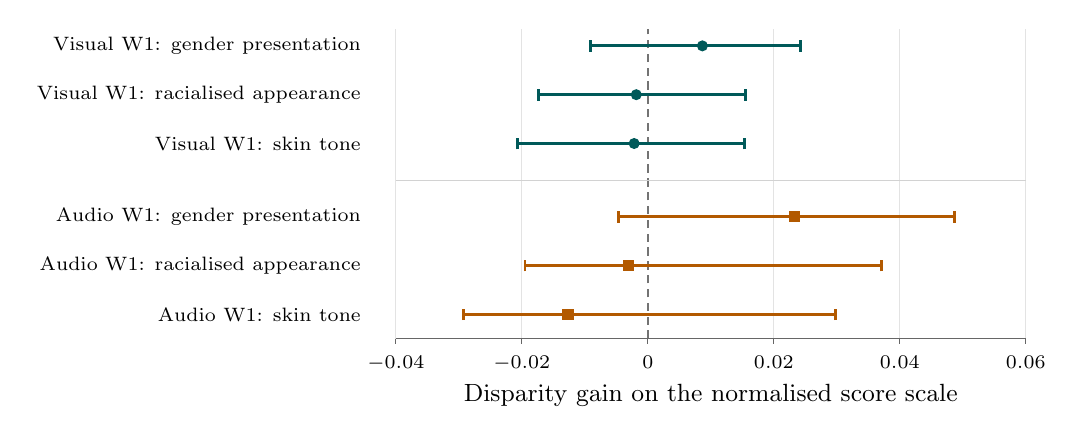
\begin{tikzpicture}[x=80cm,y=0.62cm]
  \foreach \x in {-0.04,-0.02,0.02,0.04,0.06} {
    \draw[gray!22] (\x,0.0) -- (\x,6.35);
  }
  \draw[black!55,densely dashed,line width=0.8pt] (0,0.0) -- (0,6.35);
  \draw[black!60] (-0.04,0.0) -- (0.06,0.0);
  \draw[gray!35] (-0.04,3.25) -- (0.06,3.25);

  \foreach \x/\label in {-0.04/$-0.04$,-0.02/$-0.02$,0/$0$,0.02/$0.02$,0.04/$0.04$,0.06/$0.06$} {
    \draw[black!60] (\x,0.0) -- (\x,-0.10);
    \node[font=\scriptsize,anchor=north] at (\x,-0.16) {\label};
  }
  \node[font=\small,anchor=north] at (0.01,-0.72)
    {Disparity gain on the normalised score scale};

  \node[font=\scriptsize,anchor=east] at (-0.044,6) {Visual W1: gender presentation};
  \node[font=\scriptsize,anchor=east] at (-0.044,5) {Visual W1: racialised appearance};
  \node[font=\scriptsize,anchor=east] at (-0.044,4) {Visual W1: skin tone};
  \node[font=\scriptsize,anchor=east] at (-0.044,2.5) {Audio W1: gender presentation};
  \node[font=\scriptsize,anchor=east] at (-0.044,1.5) {Audio W1: racialised appearance};
  \node[font=\scriptsize,anchor=east] at (-0.044,0.5) {Audio W1: skin tone};

  % Visual W1 versus same-seed ERM: pointwise 95% participant-cluster intervals.
  \draw[teal!70!black,line width=1pt] (-0.009153,6) -- (0.024242,6);
  \draw[teal!70!black,line width=1pt] (-0.009153,5.88) -- (-0.009153,6.12);
  \draw[teal!70!black,line width=1pt] (0.024242,5.88) -- (0.024242,6.12);
  \fill[teal!70!black] (0.008671,6) circle[radius=2pt];

  \draw[teal!70!black,line width=1pt] (-0.017332,5) -- (0.015458,5);
  \draw[teal!70!black,line width=1pt] (-0.017332,4.88) -- (-0.017332,5.12);
  \draw[teal!70!black,line width=1pt] (0.015458,4.88) -- (0.015458,5.12);
  \fill[teal!70!black] (-0.001826,5) circle[radius=2pt];

  \draw[teal!70!black,line width=1pt] (-0.020646,4) -- (0.015386,4);
  \draw[teal!70!black,line width=1pt] (-0.020646,3.88) -- (-0.020646,4.12);
  \draw[teal!70!black,line width=1pt] (0.015386,3.88) -- (0.015386,4.12);
  \fill[teal!70!black] (-0.002168,4) circle[radius=2pt];

  % Interview-audio W1 versus same-seed ERM, plotted with square markers.
  \draw[orange!70!black,line width=1pt] (-0.004588,2.5) -- (0.048720,2.5);
  \draw[orange!70!black,line width=1pt] (-0.004588,2.38) -- (-0.004588,2.62);
  \draw[orange!70!black,line width=1pt] (0.048720,2.38) -- (0.048720,2.62);
  \node[rectangle,fill=orange!70!black,minimum size=4pt,inner sep=0pt] at (0.023337,2.5) {};

  \draw[orange!70!black,line width=1pt] (-0.019508,1.5) -- (0.037087,1.5);
  \draw[orange!70!black,line width=1pt] (-0.019508,1.38) -- (-0.019508,1.62);
  \draw[orange!70!black,line width=1pt] (0.037087,1.38) -- (0.037087,1.62);
  \node[rectangle,fill=orange!70!black,minimum size=4pt,inner sep=0pt] at (-0.003113,1.5) {};

  \draw[orange!70!black,line width=1pt] (-0.029259,0.5) -- (0.029783,0.5);
  \draw[orange!70!black,line width=1pt] (-0.029259,0.38) -- (-0.029259,0.62);
  \draw[orange!70!black,line width=1pt] (0.029783,0.38) -- (0.029783,0.62);
  \node[rectangle,fill=orange!70!black,minimum size=4pt,inner sep=0pt] at (-0.012670,0.5) {};
\end{tikzpicture}

\caption{The six primary post-session three-seed mean disparity gains and pointwise 95\%
participant-cluster intervals from Table~\ref{tab:stage-c-disparity-contrasts}. The zero line
denotes no difference between each W1 configuration and same-seed ERM; positive values indicate
smaller predicted-score disparity under W1. These are perceived-attribute audit results, not
demographic-identity or hiring-fairness effects.}
\label{fig:stage-c-primary-disparity}
\end{figure}
\FloatBarrier

All six primary intervals cross zero (Figure~\ref{fig:stage-c-primary-disparity}); some
seed-specific gains also change sign. The data therefore do not resolve a reduction in any of
the three audited disparities for either W1 configuration relative to ERM. The intervals are
pointwise descriptive intervals over a fixed contrast family, without multiple-comparison
adjustment or automatic superiority tests.

Table~\ref{tab:stage-c-secondary-contrasts} gives the corresponding exploratory component and
control comparisons. Neither incremental W1 comparison with its matched sampling-only
configuration, the random-proxy comparison, ARL nor the protected-annotation oracle has a
three-seed mean disparity-gain interval excluding zero on any axis. The oracle was trained only
on the observed binary post-session perceived-gender-presentation field; it is neither a
protected-group-free method nor a performance upper bound. Its pooled original-scale MAE
improvement over ERM was $-0.068$ [$-0.108$, $-0.031$], while its pooled SRCC
change was $-0.010$ [$-0.057$, 0.032]. These contrasts do not support a
disparity--utility benefit for the oracle.

\begin{table}[htbp]
\centering
\caption{Secondary post-session three-seed mean disparity gains with pointwise 95\%
participant-cluster intervals, on the normalised 0--1 scale. Positive values denote lower
audited predicted-score W1 under the first configuration. Sampling comparisons isolate the
incremental W1 term; the remaining rows are
controls or an exploratory supervised oracle.}
\label{tab:stage-c-secondary-contrasts}
\small
\begin{adjustbox}{max width=\textwidth}
\begin{tabular}{lccc}
\toprule
Contrast & Gender presentation & Racialised appearance & Skin tone \\
\midrule
Visual W1 vs visual sampling & \shortstack{$-0.002$\\{[$-0.016$, 0.009]}} & \shortstack{$-0.006$\\{[$-0.023$, 0.012]}} & \shortstack{0.003\\{[$-0.017$, 0.017]}} \\
Audio W1 vs audio sampling & \shortstack{0.009\\{[$-0.006$, 0.022]}} & \shortstack{$-0.002$\\{[$-0.028$, 0.028]}} & \shortstack{$-0.006$\\{[$-0.022$, 0.017]}} \\
Random-proxy W1 vs ERM & \shortstack{$-0.007$\\{[$-0.029$, 0.020]}} & \shortstack{0.002\\{[$-0.027$, 0.029]}} & \shortstack{$-0.005$\\{[$-0.023$, 0.026]}} \\
ARL vs ERM & \shortstack{$-0.002$\\{[$-0.009$, 0.006]}} & \shortstack{$-0.006$\\{[$-0.023$, 0.016]}} & \shortstack{$-0.0003$\\{[$-0.013$, 0.012]}} \\
Perceived-gender oracle vs ERM & \shortstack{0.010\\{[$-0.016$, 0.032]}} & \shortstack{0.001\\{[$-0.028$, 0.018]}} & \shortstack{$-0.013$\\{[$-0.035$, 0.016]}} \\
\bottomrule
\end{tabular}
\end{adjustbox}
\end{table}
\FloatBarrier

\subsection{Proxy-to-perception association after prediction lock}

% Source: results/proxy-association-correction-2026-11-06.json.
The visual partition agrees exactly with the observer's post-session gender-presentation
codes in each outer test fold: NMI and ARI are both 1.000. The fold sizes are 14, 14, 14,
14 and 13 participants. A pooled description is possible only after resolving the
arbitrary cluster IDs. Alignment uses agreement among shared training participants,
without annotations or outcomes; it reveals the same visual partition up to a label
swap in every rotation. The aligned held-out groups contain 43 and 26 people and
retain NMI and ARI of 1.000 against this observer's gender-presentation codes.
Association with racialised appearance is much smaller (NMI 0.025, ARI 0.017;
65 known annotations), as is association with ordinal skin tone (NMI 0.012,
ARI $-0.003$; 69 annotations).

The audio partition changes beyond label swaps across rotations, so it does not support
a single pooled aligned group identity. Its fold-local held-out gender-presentation
NMI ranges from 0.002 to 0.094 and ARI from $-0.071$ to 0.026. These statistics describe
association with a single observer's perception of this corpus, not gender identity
or general demographic-classification accuracy. Perceived-group score disparities
above depend directly on annotations and are unaffected by cluster-number alignment.

\subsection{Annotation-conditioned errors}

Table~\ref{tab:stage-c-group-error} shows the reportable-category absolute errors and signed
residuals for ERM on the 69 post sessions. Each range is the minimum--maximum across fixed seeds
1, 11 and 21, \emph{not} a confidence interval. Errors are on the original 1--7 rating scale,
and residual is prediction minus target; a negative residual indicates underprediction of the
crowd rating. Categories on different axes overlap, so rows cannot be pooled as independent
subsamples. The aggregate also contains seed-specific group bootstrap intervals; this compact
table does not convert the ranges into a test of between-group error equality.

\begin{table}[htbp]
\centering
\caption{Post-session ERM error by reportable perceived category. Values are descriptive
minimum--maximum across the three fixed seeds on the original 1--7 rating scale; residual is
prediction minus crowd-perceived hireability.}
\label{tab:stage-c-group-error}
\small
\begin{adjustbox}{max width=\textwidth}
\begin{tabular}{llrrr}
\toprule
Perceived axis & Category & Participants & MAE range & Mean residual range \\
\midrule
Gender presentation & F & 43 & 0.755--1.223 & $-0.899$--$-0.240$ \\
 & M & 26 & 0.787--1.368 & $-1.161$--$-0.282$ \\
Racialised appearance & W & 24 & 0.997--1.308 & $-0.988$--$-0.431$ \\
 & EA & 16 & 0.680--1.288 & $-0.979$--$-0.112$ \\
 & MENA & 11 & 0.614--0.955 & $-0.558$--$-0.151$ \\
Skin tone & 1 & 20 & 0.880--1.316 & $-1.138$--$-0.601$ \\
 & 2 & 27 & 0.775--1.098 & $-0.762$--$-0.207$ \\
 & 3 & 15 & 0.562--1.262 & $-0.861$--0.079 \\
\bottomrule
\end{tabular}
\end{adjustbox}
\end{table}
\FloatBarrier

Absolute errors differ descriptively across these reported categories, but the same
seed-specific ranges often overlap and the small groups limit precision. Most listed ERM
residual ranges are negative. Neither pattern identifies bias against a verified demographic
group, and the suppressed categories have no error estimate.

\subsection{Pre-session sensitivity on available annotations}

The separate sensitivity uses only the 57 participants with pre-session annotations; the 12
missing pre annotations were neither imputed nor carried forward from post. This roster is not
assumed missing at random. The pre reportability pattern differs from the post pattern
(Table~\ref{tab:annotation-intake}): the reportable categories contain 57 participants for gender
presentation, 30 for racialised appearance and 44 for skin tone. Thus the maximum pairwise W1
can be attained by different category pairs. Table~\ref{tab:stage-c-pre-disparity-contrasts}
reports the same fixed contrast
family and sign convention, recomputed on the 57 pre sessions. All 21 three-seed mean pre
disparity-gain intervals cross zero. The pre results therefore do not rescue a mitigation claim
and do not estimate any causal pre/post or coaching effect.

\begin{table}[htbp]
\centering
\caption{Available-case pre-session three-seed mean disparity gains with pointwise 95\%
participant-cluster intervals ($n=57$), on the normalised 0--1 scale. Positive values denote lower
audited predicted-score W1 under the first configuration; category eligibility is recalculated
for the pre roster.}
\label{tab:stage-c-pre-disparity-contrasts}
\small
\begin{adjustbox}{max width=\textwidth}
\begin{tabular}{lccc}
\toprule
Contrast & Gender presentation & Racialised appearance & Skin tone \\
\midrule
Visual W1 vs ERM & \shortstack{0.010\\{[$-0.013$, 0.028]}} & \shortstack{$-0.005$\\{[$-0.025$, 0.018]}} & \shortstack{0.009\\{[$-0.014$, 0.027]}} \\
Audio W1 vs ERM & \shortstack{0.012\\{[$-0.010$, 0.032]}} & \shortstack{0.011\\{[$-0.015$, 0.033]}} & \shortstack{$-0.003$\\{[$-0.023$, 0.023]}} \\
Visual W1 vs visual sampling & \shortstack{0.001\\{[$-0.015$, 0.017]}} & \shortstack{0.002\\{[$-0.018$, 0.021]}} & \shortstack{0.013\\{[$-0.005$, 0.020]}} \\
Audio W1 vs audio sampling & \shortstack{0.005\\{[$-0.008$, 0.018]}} & \shortstack{0.011\\{[$-0.006$, 0.026]}} & \shortstack{0.003\\{[$-0.012$, 0.018]}} \\
Random-proxy W1 vs ERM & \shortstack{0.001\\{[$-0.022$, 0.021]}} & \shortstack{$-0.001$\\{[$-0.027$, 0.024]}} & \shortstack{$-0.002$\\{[$-0.022$, 0.019]}} \\
ARL vs ERM & \shortstack{$-0.002$\\{[$-0.009$, 0.008]}} & \shortstack{0.002\\{[$-0.011$, 0.012]}} & \shortstack{$-0.003$\\{[$-0.009$, 0.007]}} \\
Perceived-gender oracle vs ERM & \shortstack{0.013\\{[$-0.021$, 0.035]}} & \shortstack{$-0.011$\\{[$-0.032$, 0.020]}} & \shortstack{0.009\\{[$-0.019$, 0.028]}} \\
\bottomrule
\end{tabular}
\end{adjustbox}
\end{table}
\FloatBarrier

\subsection{Utility alongside audited disparity}

The six pooled-session utility contrasts and their participant-cluster intervals are reported in
Table~\ref{tab:stage-a-utility-contrasts}. They use both sessions of all 69 participants (138
held-out predictions per configuration and seed), whereas the primary perceived-attribute
disparity contrasts use one post session per participant. Reproducing pooled utility in Stage C
checks the same predictions rather than providing independent replication. For the post-only
roster, three-seed mean SRCC was 0.084 for ERM, 0.079 for visual W1 and 0.004 for
interview-audio W1; the corresponding original-scale MAEs were 1.025, 1.026 and 0.954.
These are descriptive phase-specific means, not a combined fairness--utility score or a
post-session interval comparison. The two incremental W1 contrasts had lower pooled correlation
and higher pooled errors than their matched sampling-only controls on all four utility measures.
The audio-W1 contrast with ERM had a positive pooled RMSE improvement but a negative, uncertain
SRCC change. Neither a general utility gain nor a simultaneous utility-and-disparity benefit is
supported by the fixed comparisons.

Every audited axis is a single-observer perception under the recorded video conditions, not
verified demographic identity. The source has no inter-rater agreement estimate and the
crowd-perceived target itself has low individual-rating agreement. The small category sizes,
pointwise intervals, incomplete pre wave and mixed-speaker interview audio further limit
generalisation. No result here establishes a causal coaching effect, hiring fairness,
employment-outcome validity or a legal-compliance judgement.

\section{Prediction with competitive linear scorers}
\label{sec:linear-results}

% Sources: results/study2_rq1_aggregate_v1.json; results/study2-compact-2026-10-21-aggregate.json.
The follow-up asks whether the weak original model obscured the behaviour of the penalty.
The natural-exposure linear reference reproduces the fixed all-modality ridge result:
pooled OOF SRCC 0.418 and normalised MAE 0.089 (original-scale MAE 0.535). It therefore
provides a materially stronger predictor than the original neural reference. This is not
evidence that linearity is universally preferable; it establishes a credible comparison
point for this small dataset and these frozen representations.

The separate outcome-only selection analysis chose tuned ridge in every outer rotation,
with alpha 1000 in all five. Table~\ref{tab:ridge-selection} reports the available outer-fold
summary. Its mean SRCC of 0.567 is an average of five within-fold correlations, while the
0.418 value above is calculated once from concatenated OOF predictions. These different
summaries must not be ranked as if their difference were a paired improvement estimate.
The selection summary supplies no uncertainty interval for that comparison.

\begin{table}[htbp]
\centering
\caption{Outcome-only predictive selection: unweighted means of five outer-fold metrics.
MAE uses the normalised MIT scale. These are not pooled OOF correlations.}
\label{tab:ridge-selection}
\begin{tabular}{lrr}
\toprule
Predictor & Mean fold MAE & Mean fold SRCC \\
\midrule
Phase-specific training mean & 0.096 & 0.226 \\
Selected tuned ridge & 0.081 & 0.567 \\
\bottomrule
\end{tabular}
\end{table}
\FloatBarrier

\section{Proxy response of the linear scorer}
\label{sec:compact-mechanism-results}

% Source: results/study2-compact-2026-10-21-aggregate.json.
The compact follow-up covers all 15 configurations and 75 outer-fold fits, yielding 2,070
held-out session predictions. Sixty-two fits meet their solver termination criterion.
Thirteen fits at the strongest coefficient, 0.2, reach the fixed iteration cap with finite
predictions. Every fit in the four primary strength-0.02 comparisons converged. The complete
grid in Table~\ref{tab:compact-grid} retains the capped results; those strongest-penalty
points describe bounded optimisation rather than established converged optima.

Unlike the original sampler comparison, the balanced-exposure control here evaluates the
full-fold group-weighted task objective. Its near-identical utility to natural exposure is
an observed result of this linear setting, not proof that balancing has no effect in other
models. Each W1 configuration changes only the penalty relative to its own exposure control.
All errors in the compact tables use the normalised MIT target scale.

\begin{table}[htbp]
\centering
\caption{Complete linear strength comparison on 138 pooled OOF sessions. All five test
folds are concatenated before each metric. A dagger identifies a configuration with at
least one iteration-capped fit; it is not a significance marker.}
\label{tab:compact-grid}
\small
\begin{tabular}{llrrr}
\toprule
Proxy & Task exposure & $\lambda$ & MAE & SRCC \\
\midrule
None & Natural & 0 & 0.089 & 0.418 \\
Visual & Balanced & 0 & 0.089 & 0.418 \\
Audio & Balanced & 0 & 0.089 & 0.418 \\
\addlinespace
Visual & Natural & 0.002 & 0.089 & 0.416 \\
 & & 0.02 & 0.090 & 0.389 \\
 & & $0.2^{\dagger}$ & 0.090 & 0.383 \\
Visual & Balanced & 0.002 & 0.089 & 0.416 \\
 & & 0.02 & 0.090 & 0.387 \\
 & & $0.2^{\dagger}$ & 0.089 & 0.392 \\
\addlinespace
Audio & Natural & 0.002 & 0.089 & 0.414 \\
 & & 0.02 & 0.091 & 0.374 \\
 & & $0.2^{\dagger}$ & 0.103 & 0.134 \\
Audio & Balanced & 0.002 & 0.089 & 0.414 \\
 & & 0.02 & 0.089 & 0.385 \\
 & & $0.2^{\dagger}$ & 0.103 & 0.129 \\
\bottomrule
\end{tabular}
\end{table}
\FloatBarrier

The penalty changes its intended quantity on both training and held-out proxy groups
(Table~\ref{tab:compact-manipulation}). For visual natural exposure at strength 0.02,
mean training W1 declines from 0.036 to 0.009 and mean held-out W1 from 0.045 to 0.035.
The audio natural-exposure comparison declines from 0.134 to 0.090 in training and from
0.087 to 0.068 on held-out groups. These distances are calculated within each fold's
own partition before the five distances are averaged. They establish an observed proxy
response rather than an audited-group fairness result.

\begin{table}[htbp]
\centering
\caption{Proxy manipulation at $\lambda=0.02$. Entries are arithmetic means of five
fold-specific W1 values. ``Control'' is the matched zero-penalty exposure.}
\label{tab:compact-manipulation}
\small
\begin{tabular}{llrrrr}
\toprule
Proxy & Exposure & Train control & Train W1 & Test control & Test W1 \\
\midrule
Visual & Natural & 0.036 & 0.009 & 0.045 & 0.035 \\
Visual & Balanced & 0.036 & 0.010 & 0.045 & 0.036 \\
Audio & Natural & 0.134 & 0.090 & 0.087 & 0.068 \\
Audio & Balanced & 0.134 & 0.096 & 0.087 & 0.070 \\
\bottomrule
\end{tabular}
\end{table}
\FloatBarrier

The response comes with a ranking cost. The visual natural-exposure SRCC change is
$-0.030$ with paired interval [$-0.069$, 0.008]. The audio natural-exposure change is
$-0.044$ [$-0.080$, $-0.008$]. Their normalised MAE changes are 0.001
[$-0.002$, 0.003] and 0.002 [$-0.001$, 0.005], respectively.
The balanced visual and audio SRCC changes are $-0.031$ [$-0.066$, 0.004] and
$-0.033$ [$-0.067$, 0.002]. These pointwise intervals condition on the fixed fitted
models; they do not include retraining or model-selection uncertainty. The strongest audio
coefficient also produces substantially lower point SRCC, but its capped optimisation
requires a separate numerical qualification.

\section{Transfer to perceived-group disparity}
\label{sec:compact-audit-results}

% Source: results/study2-compact-2026-10-21-aggregate.json.
The new phase-aligned audit uses the same single-observer source and reportable categories
as the original study. Its primary post roster remains 69 participants. On the working
natural-exposure reference, perceived-gender score W1 is 0.049. Visual W1 at strength 0.02
reduces the point estimate to 0.029, giving a gain of approximately 0.020. The paired
interval [$-0.005$, 0.025] includes zero, so the study does not resolve a population
reduction. The balanced visual comparison gives the same rounded gain with interval
[$-0.004$, 0.024].

Table~\ref{tab:compact-audit-gains} shows why the visual point change cannot be generalised
to every audited attribute. Racialised-appearance point gains are negative, while skin-tone
gains are small; every displayed interval crosses zero. The audio proxy also has a
smaller perceived-gender response than its own held-out proxy response would suggest.
Reducing the distance between two learned clusters therefore does not establish a
simultaneous improvement across the observer's other partitions.

\begin{table}[htbp]
\centering
\caption{Compact linear follow-up: primary post-session disparity gains at $\lambda=0.02$
relative to the exact exposure control. Positive values favour W1. Brackets are pointwise
95\% paired participant-percentile intervals; all values use the normalised score scale.}
\label{tab:compact-audit-gains}
\small
\begin{adjustbox}{max width=\textwidth}
\begin{tabular}{llccc}
\toprule
Proxy & Exposure & Gender presentation & Racialised appearance & Skin tone \\
\midrule
Visual & Natural & 0.020 [$-0.005$, 0.025] & $-0.009$ [$-0.015$, 0.010] & 0.001 [$-0.006$, 0.010] \\
Visual & Balanced & 0.020 [$-0.004$, 0.024] & $-0.007$ [$-0.013$, 0.010] & 0.001 [$-0.005$, 0.010] \\
Audio & Natural & 0.004 [$-0.002$, 0.011] & $-0.002$ [$-0.006$, 0.016] & 0.003 [$-0.002$, 0.013] \\
Audio & Balanced & 0.004 [$-0.002$, 0.010] & $-0.002$ [$-0.005$, 0.015] & 0.002 [$-0.003$, 0.012] \\
\bottomrule
\end{tabular}
\end{adjustbox}
\end{table}
\FloatBarrier

The separate 57-person pre sensitivity does not create a second observer or a replication.
Its visual perceived-gender gains are approximately 0.005, with intervals that include
zero. The audio gains are also about 0.005 and their lower interval endpoints round to
zero; this reduced, incompletely labelled phase cannot replace the primary post result.
All five ordinal skin-tone codes remain in the source counts and are not binarised.

Taken together, the linear results remove two ambiguities of the original experiment:
the comparison now uses a working predictor, and the penalty demonstrably changes the
observed proxy quantity on held-out participants. They do not remove the small-sample or
single-observer limits, and they do not establish a general disparity--utility improvement.

\section{AVI prediction and self-reported group error}
\label{sec:avi-results}

% Source: results/avi-baseline-2026-11-02-reconciled.json.
The AVI feature release covers 646 participants with six valid question clips each.
Supervised fitting uses 450 training participants; validation and test contain 64 and
130 participants. Ridge selection chooses alpha 1000, with validation MAE 0.415 on
the source 1--5 rating scale. On the official test, MAE is 0.419, compared with 0.479
for the training-target mean (Table~\ref{tab:avi-baseline}). The absolute improvement
is 0.060 rating points, approximately a 12.6\% reduction in MAE. This is a point
comparison on one held-out corpus, without a supplied paired uncertainty interval for
the utility improvement.

\begin{table}[htbp]
\centering
\caption[AVI-Personality baseline and descriptive group errors]{Independent AVI-Personality baseline on the original 1--5 interview-performance
scale. The official test contains 130 participants. Group results are descriptive.}
\label{tab:avi-baseline}
\begin{tabular}{lrr}
\toprule
Prediction or audit group & Test participants & MAE$_{1--5}$ \\
\midrule
Training-target mean reference & 130 & 0.479 \\
Validation-selected ridge & 130 & 0.419 \\
\addlinespace
Self-reported male & 67 & 0.452 \\
Self-reported female & 62 & 0.385 \\
Prefer not to say & 1 & Not estimated \\
Non-binary / third gender & 0 & Not estimated \\
\bottomrule
\end{tabular}
\end{table}
\FloatBarrier

The observed male-minus-female MAE difference is 0.067 rating points. It is a difference
in error against a recruiter rating, not in hiring outcomes or predicted-score parity.
The available absolute-gap bootstrap does not provide a signed-gap test, so the point
difference is not described as a statistically established population disparity. Sparse
and absent source categories remain visible and are not recoded to obtain an estimate.

This baseline supports the limited observation that the frozen video/audio
representations contain useful signal for a distinct interview rating. Taken on its own it
evaluates a predictive model and its group errors, without a penalised comparison; the
matched intervention and control arms reported in
Section~\ref{sec:avi-compact-results} are analysed separately below, after the baseline
and its audit had already been inspected. The raw AVI MAE is not ranked
against MIT MAE because the outcomes, scales and visual input boundaries differ.

\subsection{Matched proxy-penalty comparison on independent participants}
\label{sec:avi-compact-results}

% Source: results/avi-compact-reconciled-v1.json.
The fifteen fixed settings of Section~\ref{sec:avi-compact-method} were fitted on the same
feature release and evaluated on the official 130-participant test, giving 1{,}950 locked
prediction rows. Nine of the fifteen optimisations reported convergence; the remaining six
produced finite predictions but terminated without a convergence report. Those six are
retained in the complete grid and are described as bounded optimisation outcomes rather
than established optima. Table~\ref{tab:avi-compact-arms} gives the complete grid.

\begin{table}[htbp]
\centering
\caption[Complete AVI proxy-penalty grid]{Complete fifteen-arm grid on the independent
test. Errors are in original 1--5 rating units; score W1 is the Wasserstein-1 distance
between the predicted-score distributions of the two supported source gender groups, on the
normalised prediction scale. Prediction SD is reported against a target SD of 0.149.}
\label{tab:avi-compact-arms}
\small
\begin{adjustbox}{max width=\textwidth}
\begin{tabular}{llrrrrr}
\toprule
Proxy source & Exposure & $\lambda$ & MAE$_{1-5}$ & SRCC & Score W1 & Prediction SD \\
\midrule
None (control) & Natural & --- & 0.419 & 0.473 & 0.062 & 0.081 \\
\addlinespace
Visual & Natural & 0.002 & 0.419 & 0.473 & 0.061 & 0.081 \\
Visual & Natural & 0.02 & 0.421 & 0.455 & 0.061 & 0.080 \\
Visual & Natural & 0.2 & 0.424 & 0.445 & 0.059 & 0.078 \\
Audio & Natural & 0.002 & 0.419 & 0.473 & 0.061 & 0.081 \\
Audio & Natural & 0.02 & 0.422 & 0.442 & 0.057 & 0.074 \\
Audio & Natural & 0.2 & 0.453 & 0.295 & 0.050 & 0.067 \\
\addlinespace
Visual (control) & Balanced & --- & 0.420 & 0.463 & 0.064 & 0.083 \\
Visual & Balanced & 0.002 & 0.419 & 0.464 & 0.064 & 0.083 \\
Visual & Balanced & 0.02 & 0.417 & 0.464 & 0.065 & 0.083 \\
Visual & Balanced & 0.2 & 0.420 & 0.447 & 0.050 & 0.080 \\
\addlinespace
Audio (control) & Balanced & --- & 0.421 & 0.467 & 0.068 & 0.084 \\
Audio & Balanced & 0.002 & 0.421 & 0.466 & 0.068 & 0.083 \\
Audio & Balanced & 0.02 & 0.424 & 0.435 & 0.063 & 0.077 \\
Audio & Balanced & 0.2 & 0.462 & 0.320 & 0.054 & 0.070 \\
\bottomrule
\end{tabular}
\end{adjustbox}
\end{table}
\FloatBarrier

\subsubsection{Primary matched contrast}

The pre-specified primary contrast is the visual natural-exposure arm at $\lambda=0.02$
against its task-only control. Its original-scale MAE changes by 0.002 rating points
(95\% interval $[-0.003, 0.008]$), its rank correlation by $-0.018$
($[-0.041, 0.002]$), and its gender score-disparity gain is 0.001
($[-0.002, 0.004]$). All three intervals contain zero. On this corpus, at the strength
that served as the primary setting of the main study, the penalty therefore produced
neither a detectable utility cost nor a detectable disparity improvement.

\subsubsection{Held-out proxy response}

The penalty did act on its optimisation target. Table~\ref{tab:avi-compact-mechanism}
separates the training and held-out proxy-group W1 for each arm against its own proxy
source. In training, the visual proxy gap falls from 0.021 in the natural control to 0.003
at $\lambda=0.02$ and below 0.001 at $\lambda=0.2$, and the audio proxy gap falls from 0.118
to 0.082 and then also below 0.001. The penalty is thus doing what it is specified to do
in-sample, and the absence of a disparity effect is not an optimisation failure.

Transfer to held-out participants differs sharply between the two proxies. The visual
held-out gap falls only from 0.032 to 0.027 at $\lambda=0.02$, and stands at 0.031 at
$\lambda=0.2$ despite a training gap collapsed by more than a factor of forty. The audio
held-out gap falls substantially, from 0.074 to 0.049 and then to 0.023. The visual proxy
constraint therefore does not generalise beyond the participants it was fitted on, whereas
the audio proxy constraint does.

\begin{table}[htbp]
\centering
\caption[Training and held-out proxy response]{Wasserstein-1 distance between predicted-score
distributions of the two unsupervised proxy groups, measured against each arm's own proxy
source, on the normalised prediction scale. Visual partitions contain 368/82 training and
103/27 test participants; audio partitions contain 143/307 training and 35/95 test
participants.}
\label{tab:avi-compact-mechanism}
\small
\begin{tabular}{llrrr}
\toprule
Proxy source & Exposure & $\lambda$ & Training W1 & Held-out W1 \\
\midrule
Visual & Natural & --- & 0.021 & 0.032 \\
Visual & Natural & 0.002 & 0.018 & 0.030 \\
Visual & Natural & 0.02 & 0.003 & 0.027 \\
Visual & Natural & 0.2 & $<$0.001 & 0.031 \\
\addlinespace
Visual & Balanced & --- & 0.018 & 0.035 \\
Visual & Balanced & 0.002 & 0.016 & 0.035 \\
Visual & Balanced & 0.02 & 0.005 & 0.030 \\
Visual & Balanced & 0.2 & $<$0.001 & 0.029 \\
\addlinespace
Audio & Balanced & --- & 0.118 & 0.074 \\
Audio & Natural & 0.002 & 0.115 & 0.071 \\
Audio & Natural & 0.02 & 0.082 & 0.049 \\
Audio & Natural & 0.2 & $<$0.001 & 0.023 \\
Audio & Balanced & 0.002 & 0.115 & 0.072 \\
Audio & Balanced & 0.02 & 0.086 & 0.051 \\
Audio & Balanced & 0.2 & $<$0.001 & 0.022 \\
\bottomrule
\end{tabular}
\end{table}
\FloatBarrier

\subsubsection{Audited disparity across the complete grid}

Table~\ref{tab:avi-compact-effects} reports every matched contrast. At the weakest strength
all four arms are indistinguishable from their controls on all three measures. At
$\lambda=0.2$ the audio arms incur clear utility damage: original-scale MAE rises by 0.034
($[0.001, 0.066]$) under natural exposure and 0.041 ($[0.004, 0.077]$) under balanced
exposure, with rank correlation falling by 0.178 and 0.147 respectively, both intervals
excluding zero.

Three contrasts have disparity-gain intervals excluding zero: the balanced visual arm at
$\lambda=0.2$, with gain 0.014 ($[0.006, 0.019]$); the natural audio arm at $\lambda=0.02$,
with gain 0.005, whose lower endpoint is below 0.0001; and the balanced audio arm at
$\lambda=0.002$, whose gain and both endpoints round to zero at three decimals. These are
three of thirty-six intervals computed across twelve penalised arms and three outcome
measures, without correction for that multiplicity, and none is the pre-specified primary
contrast. Two of the three are marginal in the sense that their lower endpoints lie within
0.0001 of zero, and the third arises at the strongest penalty, where the matched rank
correlation also falls by 0.016. They are recorded because the complete grid is reported,
and they are not treated as established disparity reductions.

\begin{table}[htbp]
\centering
\caption[Matched AVI penalty contrasts]{Every penalised arm against its matched
exposure-sharing control, with 95\% paired participant-bootstrap intervals from 10{,}000
common draws. MAE changes are in original 1--5 rating units; a positive disparity gain
indicates a smaller gender score gap than the control. Intervals are pointwise, conditional
on these fitted models, and uncorrected for multiplicity.}
\label{tab:avi-compact-effects}
\small
\begin{adjustbox}{max width=\textwidth}
\begin{tabular}{llrccc}
\toprule
Proxy & Exposure & $\lambda$ & $\Delta$MAE$_{1-5}$ & $\Delta$SRCC & Disparity gain \\
\midrule
Visual & Natural & 0.002 & \shortstack{0.000\\{[$-0.001$, 0.001]}} & \shortstack{0.000\\{[$-0.005$, 0.005]}} & \shortstack{0.000\\{[$-0.000$, 0.001]}} \\
Visual & Natural & 0.02 & \shortstack{0.002\\{[$-0.003$, 0.008]}} & \shortstack{$-0.018$\\{[$-0.041$, 0.002]}} & \shortstack{0.001\\{[$-0.002$, 0.004]}} \\
Visual & Natural & 0.2 & \shortstack{0.006\\{[$-0.002$, 0.014]}} & \shortstack{$-0.028$\\{[$-0.056$, $-0.001$]}} & \shortstack{0.003\\{[$-0.001$, 0.008]}} \\
Audio & Natural & 0.002 & \shortstack{0.000\\{[$-0.001$, 0.001]}} & \shortstack{$-0.000$\\{[$-0.005$, 0.004]}} & \shortstack{0.001\\{[$-0.000$, 0.001]}} \\
Audio & Natural & 0.02 & \shortstack{0.003\\{[$-0.007$, 0.013]}} & \shortstack{$-0.031$\\{[$-0.065$, 0.000]}} & \shortstack{0.005\\{[0.000, 0.011]}} \\
Audio & Natural & 0.2 & \shortstack{0.034\\{[0.001, 0.066]}} & \shortstack{$-0.178$\\{[$-0.289$, $-0.070$]}} & \shortstack{0.012\\{[$-0.006$, 0.029]}} \\
\addlinespace
Visual & Balanced & 0.002 & \shortstack{$-0.000$\\{[$-0.001$, 0.000]}} & \shortstack{0.001\\{[$-0.004$, 0.005]}} & \shortstack{0.000\\{[$-0.000$, 0.000]}} \\
Visual & Balanced & 0.02 & \shortstack{$-0.003$\\{[$-0.008$, 0.003]}} & \shortstack{0.001\\{[$-0.018$, 0.021]}} & \shortstack{$-0.000$\\{[$-0.003$, 0.002]}} \\
Visual & Balanced & 0.2 & \shortstack{0.001\\{[$-0.011$, 0.012]}} & \shortstack{$-0.016$\\{[$-0.054$, 0.022]}} & \shortstack{0.014\\{[0.006, 0.019]}} \\
Audio & Balanced & 0.002 & \shortstack{$-0.000$\\{[$-0.001$, 0.001]}} & \shortstack{$-0.001$\\{[$-0.009$, 0.005]}} & \shortstack{0.000\\{[0.000, 0.001]}} \\
Audio & Balanced & 0.02 & \shortstack{0.003\\{[$-0.008$, 0.014]}} & \shortstack{$-0.032$\\{[$-0.064$, $-0.003$]}} & \shortstack{0.005\\{[$-0.000$, 0.010]}} \\
Audio & Balanced & 0.2 & \shortstack{0.041\\{[0.004, 0.077]}} & \shortstack{$-0.147$\\{[$-0.252$, $-0.045$]}} & \shortstack{0.014\\{[$-0.004$, 0.032]}} \\
\bottomrule
\end{tabular}
\end{adjustbox}
\end{table}
\FloatBarrier

\subsubsection{Group error and prediction spread}

Under the primary penalised arm the two supported source groups retain the error ordering
of the baseline: self-reported male respondents have original-scale MAE 0.453 and female
respondents 0.387, a signed difference of 0.016 on the normalised scale with interval
$[-0.014, 0.045]$. The matched change in that signed gap relative to the control is
$-0.000$ ($[-0.003, 0.002]$). The penalty did not redistribute error between the groups
it could be audited against.

Across the grid, predicted-score spread stays well below the spread of the ratings
themselves. The task-only control predicts with standard deviation 0.081 against a target
standard deviation of 0.149, and the strongest audio penalty reduces that to 0.067. The
shrinkage selected on validation error therefore compresses predictions to roughly half the
dispersion of the outcome before any fairness penalty is applied. Because a score-disparity
penalty operates on the separation between group prediction distributions, this compression
bounds the magnitude of any disparity change the penalty could produce, and it bounds it in
the same direction for every arm in the grid.

    \chapter{Discussion}
\label{ch:discussion}
\begin{spacing}{1.4}

\section{Prediction validity before a fairness interpretation}

The findings answer the research questions in a sequence: establish a useful predictor,
check the proxy mechanism, inspect transfer to audited groups, and distinguish the
independent corpus's evidence from a replication of mitigation. The original neural
experiment alone cannot support a broad conclusion about proxy regularisation because
its ordinary model is weaker than the simple references. Its pooled three-seed SRCC of
0.170 and original-scale MAE of 0.951 compare unfavourably with the fixed all-modality
ridge MAE of 0.535. This is an important baseline diagnosis, not evidence that every
possible fairness intervention must fail.

% Sources: results/study2-compact-2026-10-21-aggregate.json; results/study2_rq1_aggregate_v1.json.
The linear follow-up addresses that weakness without changing the frozen representations
or participant roster. Its natural task-only reference reproduces the working ridge
predictor, with pooled SRCC 0.418 and normalised MAE 0.089. The separate outcome-only
selection analysis also selects a strongly regularised ridge in every outer fold.
Its mean fold SRCC of 0.567 and mean fold MAE of 0.081 describe that selection procedure;
they cannot be compared directly with a pooled OOF correlation as a paired improvement.
A stronger point estimate is not a substitute for a common estimand and uncertainty
analysis. This distinction follows the broader small-sample evaluation problem:
cross-validation estimates can vary substantially~\cite{Varoquaux2018}, and selection
on noisy development estimates can bias apparent performance~\cite{CawleyTalbot2010}.

Prediction validity remains conditional on the rating. The MIT outcome is a crowd-perceived
hireability judgement, not employment success. Ordinal Krippendorff alpha of 0.232 among
individual raters shows a substantial measurement limitation. The strong agreement of the
EM aggregate with an unweighted session mean indicates agreement between aggregation
methods, not that either is an objective criterion. Measurement choices determine what
the subsequent audit can establish~\cite{JacobsWallach2021}. Interview criterion validity
depends on the construct and later outcome measured~\cite{Wingate2025ConstructValidity};
neither corpus here contains a job-performance criterion.

\section{What the proxy penalty changes}

The original experiment supplies one clear component result. Adding W1 to the matched
visual or audio sampler lowers predictive utility. The incremental SRCC changes are
$-0.038$ [$-0.072$, $-0.005$] for visual proxies and $-0.047$
[$-0.091$, $-0.002$] for audio proxies. Original-scale MAE also worsens relative to
each sampling-only control. The matched design therefore prevents a combined
sampling-and-penalty change from being attributed to W1 alone. The random proxy and
adversarial reweighting comparisons further show why an arbitrary regulariser cannot
automatically be credited with meaningful group structure.

% Source: results/study2-compact-2026-10-21-aggregate.json.
The working linear model makes the mechanism question more informative. At strength
0.02, visual natural-exposure W1 reduces mean training proxy distance from 0.036 to
0.009 and mean held-out distance from 0.045 to 0.035. Audio natural exposure also reduces
held-out proxy W1, from 0.087 to 0.068. Thus the intervention is active in the observed
training and test distributions. The empirical interpretation no longer rests on
assuming that a numerically small coefficient must have been ineffective.

This response is accompanied by a trade-off. The visual natural-exposure SRCC change is
$-0.030$ [$-0.069$, 0.008], and the audio natural-exposure change is $-0.044$
[$-0.080$, $-0.008$]. Error changes are smaller and less resolved. A reduction in
proxy-score distance consequently does not establish a beneficial joint change in
ranking and error. The complete strength grid is more informative than a single favourable
point: the strongest audio penalty has considerably weaker ranking, while the smallest
penalty changes little. Thirteen highest-strength fits reach the declared iteration limit,
so these points are bounded numerical outcomes rather than evidence of converged optima.

The two studies also evaluate different balancing mechanisms. The original uses cyclic
group-balanced minibatches, whereas the linear follow-up uses the corresponding full-fold
group-weighted task objective. Its balanced and natural controls have nearly identical
rounded utility, but this does not erase the original sampling result or establish that
stochastic exposure is irrelevant. The shared lesson is that the penalty must be compared
with its own matched task-only objective, optimiser and exposure policy.

\section{Why proxy response does not establish audited fairness}

% Source: results/study2-compact-2026-10-21-aggregate.json.
The compact visual intervention reduces the post-session perceived-gender W1 point
estimate from 0.049 to 0.029. Its paired gain of approximately 0.020 has interval
[$-0.005$, 0.025]. This is a plausible observed transfer to that partition, but the
data do not resolve a reduction at the population level. The other perceived axes
give a different pattern: racialised-appearance point gains are negative, and skin-tone
gains are small, with all primary intervals spanning zero. A model can narrow one
learned partition while leaving another unchanged or increasing its score distance.

This is the missing implication identified in proxy-fairness research. Surrogate
constraints require assumptions about their relationship with the groups of
interest~\cite{Gupta2018ProxyFairness}. The present clustering and score penalty do not
supply those assumptions automatically. Nor does a lower W1 answer the error-balance
question. Score-distribution parity and prediction errors are distinct properties of a
regression model~\cite{Petersen2023RiskScores}; neither alone defines the fairness of a
future hiring decision.

The original perceived-attribute comparison is consistent with that caution. All six
primary neural-model disparity-gain intervals include zero, as do the matched incremental
penalty contrasts. Small distances also occur for weak mean predictors. A nearly constant
score can make two groups look similar while failing to predict the target. The linear
follow-up is valuable because it demonstrates proxy response on a stronger predictor,
yet it still does not establish a general improvement across the audited attributes.

The observer source bounds the interpretation. Perceived gender presentation, racialised
appearance and skin tone are responses to a particular recording, not measurements of
self-identified attributes. The 57 pre/post annotation pairs show stable gender codes but
only 31 exact appearance matches and 26 exact skin-tone matches. These are repeated
conditions rated by one source, not independent raters. Evidence on contextual subjectivity
in skin-tone annotation reinforces the need for caution~\cite{Barrett2023}; it cannot
supply a missing reliability estimate for this observer. Skin tone remains a five-point
ordinal field, and the maximum pairwise score distance does not test an ordinal trend.

The complete post audit is primary because it includes all 69 participants, not because
a post rating is intrinsically more valid. The 57-person pre sensitivity has a different
support pattern and twelve missing annotations whose missingness is not assumed random.
A positive secondary point or a lower interval endpoint rounding to zero cannot replace
the uncertain primary result. Bootstrap precision does not create more independent
people or recover unobserved rater disagreement.

\section{Representation and proxy meaning}

Visual and audio features occupy different measurement boundaries. MIT visual inputs are
candidate-face crops, while its audio contains both interviewer and participant.
The audio clusters may reflect room, channel, timing and interviewer behaviour as well as
candidate speech. Calling them candidate-voice or speaker-identity groups would overstate
what the representation measures.

The visual partition agrees exactly with this observer's post-session
gender-presentation codes in each held-out fold. Training-participant-only alignment
also permits a pooled description because all visual partitions are identical up to
label permutation. It yields the same perfect association across the 69 OOF
participants. This is a partition-association result within one corpus, not a general
demographic classifier or evidence of gender identity. It nevertheless makes an
important distinction visible: training without supplied gender labels does not mean
that the visual features contain no gender-presentation information. Audio's low
fold-local gender association and changing partitions show that the same interpretation
cannot simply be assigned to every modality.

Neutral k-means identifiers also have no cross-fold identity. An unaligned concatenation
can manufacture an apparent disagreement even when partitions are identical up to a
permutation. The held-out manipulation analysis therefore keeps fold-specific groups.
It does not use the invalid stitched grouping to justify demographic meaning or to
calculate a pooled proxy effect. Score disparities calculated directly from perceived
annotations remain separate from this cluster-number issue.

The original inference-only masks provide a further bounded explanation. Removing the
training-standardised audio summary lowers ERM SRCC in every seed, by 0.325 on average,
whereas removing video or text sometimes improves error. These are dependence diagnostics
of one weak fitted model, not causal evidence about human communication or the value of
retraining with fewer modalities. Temporal averaging discards order, and zero-mask
inference may create inputs unlike those seen in training. Such diagnostics motivate
simple competitive references rather than a claim that visual behaviour or language is
generally uninformative.

\section{What the independent corpus adds}

% Source: results/avi-baseline-2026-11-02-reconciled.json.
AVI-Personality adds independent participants and a different rating source
~\cite{Zhang2026AVI}. Its official test contains 130 people, and the selected ridge
predictor has original-scale MAE 0.419 against 0.479 for the training-target mean.
The approximately 12.6\% lower error shows useful predictive signal in its audio/video
features on this test. It does not imply that its raw MAE is better than MIT's:
the target scale, recruiter judgement, interview format and visual input boundary differ.

The group-error audit adds another source distinction. Self-reported male respondents
have test MAE 0.452 and female respondents 0.385, a descriptive signed gap of 0.067
rating points. One prefer-not-to-say response and the absence of a non-binary or
third-gender test respondent limit the categories that can be estimated. Those source
categories cannot be collapsed or moved between splits to create support. The positive
lower endpoint of a bootstrap interval for an absolute gap does not establish a nonzero
signed population difference; the reported point gap is therefore kept descriptive.

This external ridge analysis does not contain a W1 treatment/control comparison.
Consequently, it supports independent interview-score prediction and group-error
description rather than confirmation that the proxy penalty transports. That boundary
is central to RQ4. An external dataset does not, by itself, convert an exploratory MIT
finding into a confirmed general method effect. A method comparison formulated after
the external baseline and audit have been inspected is also exploratory, even though
its participants are independent of MIT.

The visual representation further limits an exact replication claim. AVI features
average sampled full frames, whereas MIT uses operationally selected face crops.
The independent release supplies audio/video but no transcripts. These differences can
affect both prediction and the proxy partition. They are part of the scope of the
external procedure, not a reason to pool results as if the same outcome and inputs had
been observed twice.


\section{The matched comparison on independent participants}

% Source: results/avi-compact-reconciled-v1.json.
The matched fifteen-arm comparison supplies the treatment-versus-control evidence the
baseline could not. Its primary contrast, the visual natural-exposure penalty at the
strength that served as the main study's primary setting, changes original-scale error by
0.002 rating points, rank correlation by $-0.018$ and the audited gender score gap by
0.001. Every interval contains zero. The independent corpus therefore reproduces the
main study's central outcome rather than correcting it: at the primary strength, proxy
regularisation leaves both utility and audited disparity where it found them.

The more informative result is the separation between training and held-out proxy response.
The penalty succeeds completely on its own optimisation target, collapsing the training
visual proxy gap from 0.021 to below 0.001 at the strongest setting. Almost none of that
reduction survives on held-out participants, where the same arm leaves the gap at 0.031
against a control value of 0.032. The failure is therefore one of generalisation, not of
optimisation: the constraint is satisfied on the participants used to fit it and does not
describe the participants it is then applied to. This distinction matters for interpreting
the main study, where the same pattern appears in weaker form, and it is not visible from
utility and disparity summaries alone.

The audio proxy behaves differently and is the more instructive case. Its constraint does
generalise, reducing the held-out proxy gap from 0.074 to 0.023. If reducing a proxy-group
score gap were sufficient to reduce an audited group gap, this is the arm in which the
effect should appear. It does not: the corresponding disparity gain is 0.012 with interval
$[-0.006, 0.029]$, while original-scale error rises by 0.034 and rank correlation falls by
0.178, both with intervals excluding zero. A proxy constraint that transfers successfully
to new participants thus purchased a substantial utility loss without a demonstrable
fairness return. This is direct evidence that the unsupervised partition is not a usable
stand-in for the attribute the audit measures, and it is stronger evidence than a null
obtained from a constraint that never transferred at all.

Three of the thirty-six intervals across the twelve penalised arms exclude zero on the
disparity measure. None is the primary contrast, no correction was applied for examining
twelve arms on three measures, and two of the three have lower endpoints within 0.0001 of
zero. The remaining one occurs at the strongest penalty, where ranking utility is also
declining. Treating any of these as a mitigation result would be selecting an outcome
after seeing it. They are reported because the complete grid is reported, and they are
interpreted as consistent with multiplicity rather than with a located effect.

One structural feature bounds all of these comparisons. Validation-selected shrinkage leaves
predicted scores with a standard deviation of 0.081 against an outcome standard deviation
of 0.149, before any penalty is applied. A score-disparity penalty acts on the separation
between two group prediction distributions, so a predictor compressed to roughly half the
dispersion of its target offers correspondingly little separation to remove. The regularisation
strength was selected at the upper limit of its search range in every fold of every study
reported here, which indicates a shrinkage-dominated regime rather than a boundary chosen
among competitive alternatives. The absence of disparity movement is consequently
consistent with two explanations that this evidence cannot separate: that proxy
regularisation does not reduce audited disparity, or that the scorers available to it
were too compressed for any such reduction to be expressed. The second explanation is
reinforced by the main study, where the learned configurations did not reach the utility of
the deterministic ridge floors, and by the random-proxy control, which performed as well as
the structured proxies.

\section{Answering the research questions}

\textbf{RQ1, whether a participant-safe benchmark supports a competitive scorer.} Partly,
and less well than intended. Correct pairing, a reliable-enough aggregated target and a
participant-grouped evaluation were established, and the deterministic floors demonstrate
recoverable signal, reaching rank correlation 0.424 and original-scale error 0.535 on MIT
and 0.473 and 0.419 on the independent corpus. The learned configurations did not match
those floors on any of the four utility measures. The benchmark is therefore sound as a
measurement instrument while the learned scorer built on it is not competitive, and that
gap conditions every answer that follows.

\textbf{RQ2, whether proxy regularisation measurably changes held-out proxy-score
distributions beyond balanced sampling.} Only partly, and the answer depends on the proxy.
In training the penalty controls the proxy gap completely, on both corpora. On held-out
participants the visual constraint barely transfers, while the audio constraint transfers
substantially. Balanced sampling alone did not reproduce the training effect. The mechanism
is therefore real but unreliable, and its reliability is a property of the specific
representation partitioned rather than of the method.

\textbf{RQ3, whether proxy change is accompanied by changes in perceived-group disparity at
an explicit utility cost.} No. On MIT the paired disparity intervals include zero, and on
the independent corpus the primary contrast does likewise. Where a proxy constraint did
transfer, the utility cost materialised without the disparity benefit. The utility cost is
thus demonstrable and the fairness return is not, which is the opposite of the trade-off the
method is intended to offer.

\textbf{RQ4, whether the evidence transports to an independent corpus.} The null transports;
a mitigation effect does not, because none was established to transport. The independent
comparison reproduces the main study's outcome under a different outcome construct, rating
source and visual boundary, which strengthens the negative finding. It does not convert any
exploratory result into a confirmed general effect, and the comparison was itself specified
after the external baseline had been inspected.

\section{Internal and statistical validity}

Participant isolation is essential in both corpora. The corrected MIT mapping keeps
each person's pre and post recording in one fold; AVI keeps all six responses in one
official participant split. Cross-fitting nevertheless reuses participants across training
sets, so folds and training seeds are not independent experimental samples. Dependence
also complicates general cross-validation uncertainty~\cite{BengioGrandvalet2004}.

The participant bootstrap conditions on the fitted models and observed splits. Its
paired draws preserve configuration matching, but it does not estimate the variability
of retraining and selecting a model on a fresh sample. Intervals are pointwise rather
than simultaneous guarantees across the full strength, proxy and audit grid. Fairness
measurement itself can have finite-sample bias~\cite{Lum2022}; neither a nonnegative
distance nor an absolute-gap interval is a general null test.

The strongest-penalty numerical terminations, mixed-speaker MIT audio, full-frame AVI
inputs, source-label missingness and low rating agreement are substantive limits.
The input and label separation protects the declared fit from direct audit selection;
it cannot remove bias already encoded upstream or validate the target against
employment outcomes. The reciprocal source correction for two MIT post sessions is
likewise a prerequisite for valid participant analysis rather than an independent
contribution to mitigation.

\section{Practical limits and further evidence}

The research audits scores in mock-interview datasets. It does not construct or
validate a hiring tool. Outcome prediction, score-distribution similarity and observed
group error must remain separate from job-performance validity, discrimination
experienced by applicants and compliance conclusions.

The most informative further evidence would address the limits exposed here: independently
documented perceived-attribute judgements, better outcome reliability, and an external
matched intervention comparison with a credible predictor. None can be replaced by
adding more seeds, bootstrap draws or weak model variants. Candidate-speech separation
and temporal modelling are also distinct experiments rather than retrospective repairs
of these results. The supported conclusion is an active proxy mechanism with a
conditional predictive cost and uncertain audited transfer, alongside an independent
demonstration of interview-score prediction.

\end{spacing}

    \chapter{Conclusion}
\label{ch:conclusion}

This thesis examined a practical question in interview-score modelling: does making a
predictor's scores more similar across learned visual or audio groups also reduce
disparity across independently supplied attributes, without losing useful prediction?
The answer requires separating predictive validity, proxy response and audited-group
transfer. None can be inferred from a small score-distribution distance alone.

The MIT experiment uses 138 recordings from 69 correctly paired participants. Its
outcome is crowd-perceived hireability, not employment success, and the low agreement
among individual raters remains a substantive measurement limit. The original neural
scorer is weaker than the ridge references. Within that design, adding a W1 penalty
to either matched sampling control lowers rank correlation, and none of the six
primary perceived-attribute disparity contrasts resolves a reduction. This is a
controlled negative result for the evaluated model, not a general rejection of proxy
regularisation.

The exploratory linear follow-up makes the mechanism test more informative. Its
task-only scorer achieves pooled SRCC 0.418 and normalised MAE 0.089 on the same
predictions for participants held out together across sessions. At penalty strength 0.02, the visual intervention
reduces mean held-out proxy W1 from 0.045 to 0.035; the corresponding audio intervention
reduces it from 0.087 to 0.068. Thus a working predictor can respond to the proxy
constraint. The full strength grid also exposes the predictive cost rather than
selecting a favourable point after inspecting the audit. All primary-strength fits
converge, while some strongest-penalty fits reach the iteration limit.

Transfer to the perceived attributes is less certain. The visual intervention lowers
the post-session perceived-gender W1 point estimate from 0.049 to 0.029, but its
paired reduction interval includes zero. Other appearance axes do not show a consistent
benefit. The annotations describe one observer's perception of particular recordings;
they do not establish demographic identity or inter-rater reliability. Visual proxy
partitions agree with this observer's gender-presentation codes in the held-out folds,
but that association is not a general demographic-classification result. The central
finding is therefore an active proxy mechanism with a conditional utility cost and
uncertain transfer across audited groups, not demonstrated hiring fairness.

AVI-Personality extends the evidence to independent participants and recruiter-rated
interview performance. A video/audio ridge predictor achieves test MAE 0.419 on its
1--5 scale, compared with 0.479 for the training-target mean. Its observed self-reported
male--female error difference is 0.067 rating points and remains descriptive.

A matched fifteen-arm comparison on those independent participants then supplies the
treatment-versus-control evidence the baseline alone could not. At the primary strength
the penalty changes original-scale error by 0.002, rank correlation by $-0.018$ and the
audited gender score gap by 0.001, with every interval containing zero. The independent
corpus therefore reproduces the main study's outcome under a different outcome construct
and rating source rather than revising it. Separating training from held-out proxy
response makes the reason legible: the penalty collapses the training visual proxy gap
almost entirely while leaving the held-out gap essentially unchanged, so the constraint is
satisfied on the participants used to fit it and does not describe those it is applied to.
The audio proxy constraint does transfer, reducing the held-out proxy gap by two thirds,
and still yields no demonstrable disparity benefit while incurring clear utility damage.
A proxy whose constraint generalises is therefore still not a usable stand-in for the
audited attribute. Because the comparison was specified after the external baseline had
been inspected, it is exploratory on independent people rather than confirmatory, and
different outcomes, full-frame rather than face-crop video and the absence of transcripts
continue to prevent an exact replication claim.

One limitation conditions all of these results and is stated here rather than left to be
inferred. Validation-selected shrinkage reached the upper limit of its search range in
every fold of every study reported here, leaving predicted scores with roughly half the
dispersion of the ratings they predict. A score-disparity penalty acts on the separation
between group prediction distributions, so a compressed predictor offers little separation
for it to remove. The absence of disparity movement is accordingly consistent with two
explanations this evidence cannot separate: that proxy regularisation does not reduce
audited disparity, or that the scorers available to it were too compressed for such a
reduction to be expressed. The learned configurations' failure to reach the deterministic
ridge floors, and the random-proxy control's equivalence to the structured proxies, both
favour the second as a contributing factor.

The contribution is a coherent empirical distinction between predicting a subjective
interview rating, manipulating a learned partition and improving a separately audited
group metric, together with evidence that the second does not deliver the third even when
it succeeds on held-out participants. Matched task-only controls, complete
penalty-strength reporting and the separation of training from held-out proxy response
make that distinction observable. Stronger evidence would require a scorer competitive
with its own deterministic floors, a regularisation search that does not terminate at its
boundary, more reliable measurement and replication across adequately supported groups.
The present findings justify those specific tests, while providing no basis for automated
hiring, causal coaching or employment-validity claims.


    % References
    \bibliographystyle{IEEEtran}
    {\small
        \bibliography{refs}
    }

    % Appendices
    \appendix
    \chapter{Reproducibility}
\label{app:reproducibility}

This appendix gives the information needed to inspect the reported analyses and distinguish a
repeatable code check from independent empirical replication. The full corpus and row-level
annotations are restricted. Detailed technical provenance is preserved in the project record;
this appendix focuses on the study design and evidence a reader needs to assess.

\section{Data provenance and analysis units}

The study uses the MIT Interview mock-interview distribution described by Naim et
al.~\cite{Naim2015}. Its later analysis established the interview-performance prediction
setting~\cite{Naim2018}. The present distribution contains 138 audiovisual sessions, 138
non-empty transcripts and one aggregate outcome per session. The 69 participants each have a
pre and post recording. A complete face and identity audit established the participant mapping
used by this thesis. It corrects the reciprocal post-session source assignments for participants
32 and 33 while leaving the raw files and their identifiers unchanged. Data joins use raw source
identifiers; folds and paired analyses use the corrected participant identifiers.

The primary outcome is the supplied aggregate \emph{RecommendHiring} rating. A raw rating on
the documented 1--7 scale is transformed to $[0,1]$ as $(y-1)/6$ before fitting. The raw
rating, aggregate row and transformed target are kept together for every session. Individual
crowd ratings are used only in the separate target-measurement audit. No job-performance or
employment outcome is available.

Before modelling, each of the 138 sessions passed the declared audio, video, transcript and
outcome joins. All 69 complete participant pairs met the three-modality eligibility rule. No
session was imputed or replaced with a legacy feature. The independent evaluation and resampling
unit is therefore the participant, not the session.

\section{Frozen representations}

Visual input is sampled from candidate-valid face crops selected by the one-hertz, centrally
located face rule in Chapter~\ref{ch:methodology}. At most 128 crops from each session enter
DINOv2-large. The complete face manifest covers every source session and all 17,664 selected
crops; the identity audit separately checked the participant-pair mapping. The positional face
rule is an operational candidate selector, not identity recognition.

Interview audio is the bounded 16-kHz mono signal from the same active interval as visual
sampling. It contains candidate and interviewer speech because the supplied channels do not
isolate speakers. WavLM-Base+ processes at most 16 selected non-overlapping 20-second windows.
Candidate-only transcript turns, selected by the audited role parser, are encoded with the
fixed all-mpnet-base-v2 sentence-transformer checkpoint. The corpus-wide text check found 77
retained and three excluded colonless fragments under the declared continuation rule.

All three encoders remain frozen. Their versions, preprocessing settings and output dimensions
were fixed for the accepted feature set. The same representations supply every fitted
configuration, so a comparison of
training objectives does not silently substitute another modality or checkpoint.

\section{Participant-safe fitting and model contrasts}

The fixed assignment places all 69 participant pairs into five folds of sizes 14, 14, 14, 14
and 13. Both sessions from one participant always share a fold. In each outer rotation, one
fold is held out for testing, the following fold is used for stopping, and the remaining
three are used for fitting. The assignment is deterministic and independent of outcomes and
perceived-attribute annotations; its exact recipe is retained in the provenance register.

Seven ordinary configurations were fitted at seeds 1, 11 and 21 in all five rotations:
ERM, visual-proxy sampling, interview-audio-proxy sampling, random-proxy W1,
visual-proxy W1, interview-audio-proxy W1 and ARL. These yield 105 learned fits.
Nine deterministic reference predictors use the same held-out roster but do not add seeded
fits. The separate perceived-gender-presentation oracle adds 15 fits after the ordinary
predictions are fixed. Every configuration--seed combination has one out-of-fold prediction
for each of the 138 sessions. Training-only scalers, proxy centres and stopping information
are not estimated from a held-out participant. The architecture, optimiser, sampler, penalty
and stopping rule are specified in Chapter~\ref{ch:methodology}.

The two principal W1 comparisons with ERM estimate the combined effect of proxy-balanced
sampling and the W1 penalty under this fixed design. Comparisons with the corresponding
sampling-only models isolate the incremental penalty. The random partition and ARL serve
different control questions. These contrasts do not assume that an unsupervised proxy group
is a demographic group.

\section{Perceived-attribute audit}

The accepted annotation source contains one observer's session-level judgements for all 69
post sessions and 57 pre sessions. It was supplied after ordinary model predictions and proxy
assignments were fixed. The ordinary model-fitting path had no access to those fields. The
exploratory oracle uses only the observed post-session F/M perceived-gender-presentation
codes for training participants in each rotation; held-out participant annotations remain
unavailable to the oracle. This field was selected after receipt of the source, so the
oracle is not a preregistered efficacy ceiling.

The primary audit joins the 69 post predictions to their corresponding post annotations.
The incomplete 57-session pre roster is a separate sensitivity, joined only to pre
predictions. A category requires at least ten distinct participants in its phase to
support a reported disparity estimate. Unknown and smaller categories are counted but not
merged to pass this rule. Perceived skin tone remains an ordinal 1--5 field, not a binary
attribute. The single-observer source lacks inter-rater agreement and cannot establish
participants' self-identified attributes.

\section{Statistical reproduction and interpretation}

For each original model and seed, correlations and errors are recomputed once from all five
concatenated held-out folds. Fold metrics are not averaged. A mean and sample standard
deviation across the three fixed seeds describe optimisation sensitivity, not uncertainty
over independent participants. The participant-cluster bootstrap samples whole participant
records with replacement 10,000 times at its fixed seed. For pooled utility, both sessions
remain together; for the primary audit, each sampled participant contributes the matching
post prediction and annotation. Intervals for the incomplete pre roster are computed
separately.

The maximum pairwise empirical W1 distance is calculated only among reportable categories
on each perceived-attribute axis. Within-seed configuration differences are formed first;
their arithmetic mean is then recomputed in each participant resample. Reported 95\%
percentile intervals are pointwise and are not simultaneous guarantees across all axes,
configurations and seeds. The target's own group distances and category-specific errors
are reported beside predicted-score disparity so that lower W1 is not mistaken for
predictive validity or hiring fairness.

\section{Exploratory linear follow-up}

The linear mechanism comparison reuses the accepted MIT features and participant folds,
not newly extracted representations. Its 15 deterministic configurations comprise a
natural task-only ridge reference, two proxy-balanced task-only references and visual
or audio W1 at strengths 0.002, 0.02 and 0.2 under both task exposures. Five outer
rotations yield 75 fits. Natural and balanced objectives use full-fold weights rather
than replaying the neural experiment's stochastic minibatches. The initial solution
is the exact task-only ridge optimum; the score output is linear and unclipped.

The empirical W1 integrates step quantiles exactly for unequal group sizes. Optimisation
uses the training design's row space and a fixed 1,000-iteration cap. Termination states
are retained: 62 fits converge and 13 highest-strength fits reach the cap. All 20 fits
underlying the four primary strength-0.02 comparisons converge. Pooled utility is
recomputed from concatenated OOF predictions, whereas proxy manipulation is the mean
of five fold-local W1 distances. Those summaries answer different questions and are
not interchangeable. Perceived-attribute contrasts use the same 69-post/57-pre source
and paired participant bootstrap as the original audit.

A separate outcome-only ridge-selection summary reports an unweighted mean of
five outer-fold metrics after participant-grouped inner selection. Its mean fold
correlation is not a pooled OOF correlation. The available summary does not supply
a paired participant interval against the fixed-alpha compact reference. This
descriptive result is therefore reported separately rather than used to declare
a statistically established improvement.

Proxy-association analysis also respects fold identities. Visual cluster IDs are aligned
using only shared training participants, before comparison with annotations. The
partitions agree up to permutation, permitting pooled own-test-fold association.
Audio partitions do not remain identical after relabelling and are reported fold-locally.
This analysis reuses frozen assignments and does not refit models or alter the
annotation-defined score disparities.

\section{Independent-corpus evidence}

AVI-Personality preserves its official participant splits: 452 training, 64 validation
and 130 test people. All 646 have six audio/video feature vectors; two missing training
outcomes reduce supervised fitting to 450. Equal-weight averaging across six question
clips precedes participant modelling. The visual encoder receives full frames rather
than MIT's face crops, and no text representation is supplied. These differences and
the original 1--5 recruiter-rating scale are part of the external analysis definition.

Featurewise scaling is fitted on training people only. Ridge alpha is selected by
validation MAE from the fixed five-value grid, without fitting on validation or test
participants. The final predictions are clipped to the source range. The independent
test baseline and self-reported-group MAEs are descriptive accepted summaries; no
paired utility-improvement interval or signed group-gap interval is supplied.
An absolute-gap percentile interval is not used as a signed disparity test.
The external baseline has no matched W1 intervention and must not be presented
as confirmation of mitigation.

\section{Seed-specific predictive utility}

Table~\ref{tab:stage-a-seeds} preserves every learned configuration's pooled held-out
utility at each fixed seed. These are repeated computations on the same 69 participants,
not 21 independent samples. Errors are in original 1--7 rating-scale units; normalised
errors equal these values divided by six, before display rounding.

\begin{table}[H]
\centering
\caption{Seed-specific pooled out-of-fold utility for the seven learned configurations. Each row
contains one metric calculation over all 138 held-out sessions; it is not an average of fold
metrics.}
\label{tab:stage-a-seeds}
\small
\renewcommand{\arraystretch}{1.05}
\begin{tabular}{llrrrr}
\toprule
Configuration & Seed & SRCC & Pearson & MAE (1--7) & RMSE (1--7) \\
\midrule
ERM & 1 & 0.110 & 0.110 & 0.926 & 1.151 \\
ERM & 11 & 0.089 & 0.093 & 1.189 & 1.488 \\
ERM & 21 & 0.311 & 0.296 & 0.737 & 0.922 \\
Face sampling & 1 & 0.078 & 0.071 & 0.977 & 1.218 \\
Face sampling & 11 & 0.174 & 0.191 & 0.990 & 1.223 \\
Face sampling & 21 & 0.325 & 0.310 & 0.779 & 0.954 \\
Audio sampling & 1 & 0.043 & 0.055 & 0.896 & 1.133 \\
Audio sampling & 11 & 0.108 & 0.133 & 0.965 & 1.191 \\
Audio sampling & 21 & 0.327 & 0.316 & 0.733 & 0.908 \\
Random W1 & 1 & 0.101 & 0.093 & 0.971 & 1.196 \\
Random W1 & 11 & 0.190 & 0.205 & 1.129 & 1.402 \\
Random W1 & 21 & 0.296 & 0.287 & 0.700 & 0.879 \\
Face W1 & 1 & 0.072 & 0.066 & 0.987 & 1.229 \\
Face W1 & 11 & 0.098 & 0.113 & 1.140 & 1.438 \\
Face W1 & 21 & 0.294 & 0.273 & 0.740 & 0.928 \\
Audio W1 & 1 & -0.007 & 0.006 & 0.969 & 1.199 \\
Audio W1 & 11 & 0.065 & 0.094 & 0.983 & 1.213 \\
Audio W1 & 21 & 0.280 & 0.253 & 0.728 & 0.909 \\
ARL & 1 & 0.072 & 0.082 & 0.908 & 1.130 \\
ARL & 11 & 0.087 & 0.093 & 1.193 & 1.490 \\
ARL & 21 & 0.312 & 0.298 & 0.738 & 0.923 \\
\bottomrule
\end{tabular}
\end{table}

\section{Evidence integrity and reader checks}

The accepted MIT production feature release completed all 138 sessions without a structured
failure. The accepted Stage-A release contains the 105 learned fits and nine deterministic
reference predictors; its exact resume check created no additional fit. Separate
annotation-free reports cover participant-bootstrap utility, proxy diagnostics, boundary
coverage, paired-change accuracy and inference-only modality masks. Stage B's 15 oracle
fits and the phase-aligned Stage-C aggregate were completed after the declared annotation
release. These outputs were frozen before this manuscript was revised. Earlier diagnostic
or preprocessing versions that failed the accepted boundary are not used as result
sources. The project record preserves the detailed version history needed to verify those
distinctions. The exploratory linear extension and independent AVI baseline remain
separate analyses with their own evidence and measurement boundaries; they do not
replace the original predictions.

A reader with only the manuscript can inspect the analysis units, fixed comparisons,
category counts, numerical tables and interpretation limits. A reader with the project
code can run its tests and rebuild the manuscript without raw media. Recomputing
participant-level empirical outputs requires authorised access to the original corpus,
annotation source, pinned encoders and frozen run inputs. The restricted participant-level
join and identifiable media are not publication artefacts; the aggregate Stage-C report
suffices to check the reported disparity tables and figure without rerunning the audit.


\end{document}
